\PassOptionsToPackage{unicode=true}{hyperref} % options for packages loaded elsewhere
\PassOptionsToPackage{hyphens}{url}
\documentclass[11pt,dvipsnames,ignorenonframetext,aspectratio=169]{beamer}
\IfFileExists{pgfpages.sty}{\usepackage{pgfpages}}{}
\setbeamertemplate{caption}[numbered]
\setbeamertemplate{caption label separator}{: }
\setbeamercolor{caption name}{fg=normal text.fg}
\beamertemplatenavigationsymbolsempty
\usepackage{lmodern}
\usepackage{amssymb,amsmath}
\usepackage{ifxetex,ifluatex}
\usepackage{fixltx2e} % provides \textsubscript
\ifnum 0\ifxetex 1\fi\ifluatex 1\fi=0 % if pdftex
  \usepackage[T1]{fontenc}
  \usepackage[utf8]{inputenc}
\else % if luatex or xelatex
  \ifxetex
    \usepackage{mathspec}
  \else
    \usepackage{fontspec}
\fi
\defaultfontfeatures{Ligatures=TeX,Scale=MatchLowercase}







\fi

  \usetheme[]{monash}

  \usecolortheme{monashwhite}


% A default size of 24 is set in beamerthememonash.sty
  \setbeamerfont{title}{series=\bfseries,parent=structure,size=\fontsize{18pt}{32}}

% Title page
\setbeamertemplate{title page}
{\placefig{-0.01}{-0.01}{width=1.01\paperwidth,height=1.01\paperheight}{dragonfly.png}
\begin{textblock}{7.5}(1,2.8)\usebeamerfont{title}
{\color{white}\raggedright\par\inserttitle}
\end{textblock}
\begin{textblock}{7.5}(1,7)
{\color{white}\raggedright{\insertauthor}\mbox{}\\[0.2cm]
\insertdate}
\end{textblock}}


  \useinnertheme{rounded}

  \useoutertheme{smoothtree}

% use upquote if available, for straight quotes in verbatim environments
\IfFileExists{upquote.sty}{\usepackage{upquote}}{}
% use microtype if available
\IfFileExists{microtype.sty}{%
  \usepackage{microtype}
  \UseMicrotypeSet[protrusion]{basicmath} % disable protrusion for tt fonts
}{}


\newif\ifbibliography


\hypersetup{
      pdftitle={Gene Isolation and Manipulation},
            colorlinks=true,
    linkcolor=red,
    citecolor=Blue,
    urlcolor=lightgrayd,
    breaklinks=true}
%\urlstyle{same}  % Use monospace font for urls







% Prevent slide breaks in the middle of a paragraph:
\widowpenalties 1 10000
\raggedbottom

  \AtBeginPart{
    \let\insertpartnumber\relax
    \let\partname\relax
    \frame{\partpage}
  }
  \AtBeginSection{
    \ifbibliography
    \else
      \let\insertsectionnumber\relax
      \let\sectionname\relax
      \frame{\sectionpage}
    \fi
  }
  \AtBeginSubsection{
    \let\insertsubsectionnumber\relax
    \let\subsectionname\relax
    \frame{\subsectionpage}
  }



\setlength{\parindent}{0pt}
\setlength{\parskip}{6pt plus 2pt minus 1pt}
\setlength{\emergencystretch}{3em}  % prevent overfull lines
\providecommand{\tightlist}{%
  \setlength{\itemsep}{0pt}\setlength{\parskip}{0pt}}

  \setcounter{secnumdepth}{0}


%% Monash overrides
\AtBeginSection[]{
   \frame<beamer>{
   \frametitle{Outline}\vspace*{0.2cm}
   
   \tableofcontents[currentsection,hideallsubsections]
  }}

% Redefine shaded environment if it exists (to ensure text is black)
\ifcsname Shaded\endcsname
  \definecolor{shadecolor}{RGB}{225,225,225}
  \renewenvironment{Shaded}{\color{black}\begin{snugshade}\color{black}}{\end{snugshade}}
\fi
%%

  \usepackage{setspace}
  \usepackage{wasysym}
  % \usepackage{footnote} % don't use this this breaks all
  \usepackage{fontenc}
  \usepackage{fontawesome}
  \usepackage{booktabs,siunitx}
  \usepackage{longtable}
  \usepackage{array}
  \usepackage{multirow}
  \usepackage{wrapfig}
  \usepackage{float}
  \usepackage{colortbl}
  \usepackage{pdflscape}
  \usepackage{tabu}
  \usepackage{threeparttable}
  \usepackage{threeparttablex}
  \usepackage[normalem]{ulem}
  \usepackage{makecell}
  \usepackage{xcolor}
  \usepackage{tikz} % required for image opacity change
  \usepackage[absolute,overlay]{textpos} % for text formatting
  \usepackage{chemfig}
  \usepackage[skip=0.333\baselineskip]{caption}
  % \newcommand*{\AlignChar}[1]{\makebox[1ex][c]{\ensuremath{\scriptstyle#1}}}%

  % this font option is amenable for beamer
  \setbeamerfont{caption}{size=\tiny}
  \singlespacing
  \definecolor{lightgrayd}{gray}{0.95}
  \definecolor{skyblued}{rgb}{0.65, 0.6, 0.94}
  \definecolor{oranged}{RGB}{245, 145, 200}

  % \newlength{\cslhangindent}
  % \setlength{\cslhangindent}{1.5em}
  % \newenvironment{cslreferences}%
  %   {\setlength{\parindent}{0pt}%
  %   \everypar{\setlength{\hangindent}{\cslhangindent}}\ignorespaces}%
  %   {\par}
    
  \newlength{\cslhangindent}
  \setlength{\cslhangindent}{1.5em}
  \newenvironment{CSLReferences}%
  {\setlength{\parindent}{0pt}%
  \everypar{\setlength{\hangindent}{\cslhangindent}}\ignorespaces}%
  {\par}

  \newcommand{\bcolumns}{\begin{columns}[T, onlytextwidth]}
  \newcommand{\ecolumns}{\end{columns}}

  \newcommand{\bdescription}{\begin{description}}
  \newcommand{\edescription}{\end{description}}

  \newcommand{\bitemize}{\begin{itemize}}
  \newcommand{\eitemize}{\end{itemize}}
  \AtBeginSubsection{}

  \title[]{Gene Isolation and Manipulation}


  \author[
        Deependra Dhakal\\
Agriculture and Forestry University\\
\textit{ddhakal.rookie@gmail.com}\\
\url{https://rookie.rbind.io}
    ]{Deependra Dhakal\\
Agriculture and Forestry University\\
\textit{ddhakal.rookie@gmail.com}\\
\url{https://rookie.rbind.io}}


\date[
      Academic year: 2022-2023
  ]{
      Academic year: 2022-2023
        }

\begin{document}

% Hide progress bar and footline on titlepage
  \begin{frame}[plain]
  \titlepage
  \end{frame}


   \frame<beamer>{
   \frametitle{Outline}\vspace*{0.2cm}
   
   \tableofcontents[hideallsubsections]
  }

\hypertarget{manipulation-of-dna}{%
\section{Manipulation of DNA}\label{manipulation-of-dna}}

\begin{frame}{}
\protect\hypertarget{section}{}
\begin{itemize}
\tightlist
\item
  DNA manipulation includes

  \begin{itemize}
  \tightlist
  \item
    Extraction of DNA,
  \item
    Digestion of DNA,
  \item
    Fractionation of DNA,
  \item
    Synthesis of clone,
  \item
    DNA hybridization,
  \item
    DNA amplification through polymerase chain reaction,
  \item
    Recombination of DNA (genetic engineering).
  \end{itemize}
\end{itemize}
\end{frame}

\begin{frame}{}
\protect\hypertarget{section-1}{}
\begin{itemize}
\tightlist
\item
  Joining together of DNA segments from two different species is known
  as recombinant DNA technology. The rDNA technology involves:

  \begin{enumerate}
  \tightlist
  \item
    Generating a series of DNA fragments
  \item
    Joining the fragments to a carrier DNA molecule which must be able
    to replicate `vector-bacterial plasmid'
  \item
    Transforming cells with the recombinant molecule
  \end{enumerate}
\end{itemize}
\end{frame}

\hypertarget{locating-physical-position-of-dna-in-situ-hybridization}{%
\section{Locating physical position of DNA (In situ
hybridization)}\label{locating-physical-position-of-dna-in-situ-hybridization}}

\begin{frame}{}
\protect\hypertarget{section-2}{}
\begin{itemize}
\tightlist
\item
  A probe is a small, fluorescently or radioactively labeled DNA
  molecule that is used to locate similar or complementary sequences
  among a long stretch of DNA molecule or bacterial colonies such as
  genomic or cDNA libraries or in a genome.
\item
  Commonly used probe labels are radioactivity and fluorescence.
\item
  Previously, detection of nucleic acids (DNA) relied on labeling with
  radioactive isotopes (32P and 35S) incorporated into the DNA backbone
  \textbf{during replication}. Autoradiography identifies the
  radioactively labeled ``hot'' DNA.
\item
  Now used, fluorescently tagged nucleotides make use of fluorescent
  tags (Figure \ref{fig:fluorescent-tags}) that absorb light of one
  wavelength, which excites the atoms, increasing the energy state of
  the tag. This excited state releases a photon of light at a different
  (longer) wavelength and returns to ground state which is detected with
  a photodetector.
\item
  In fluorescently labeled probes ddNTPs are used in the reaction
  mixture. Each type of ddNTPs is labeled with a specific color and can
  be detected directly from the gel when illuminated with a laser or UV
  light.
\end{itemize}
\end{frame}

\begin{frame}{}
\protect\hypertarget{section-3}{}
\begin{figure}

{\centering 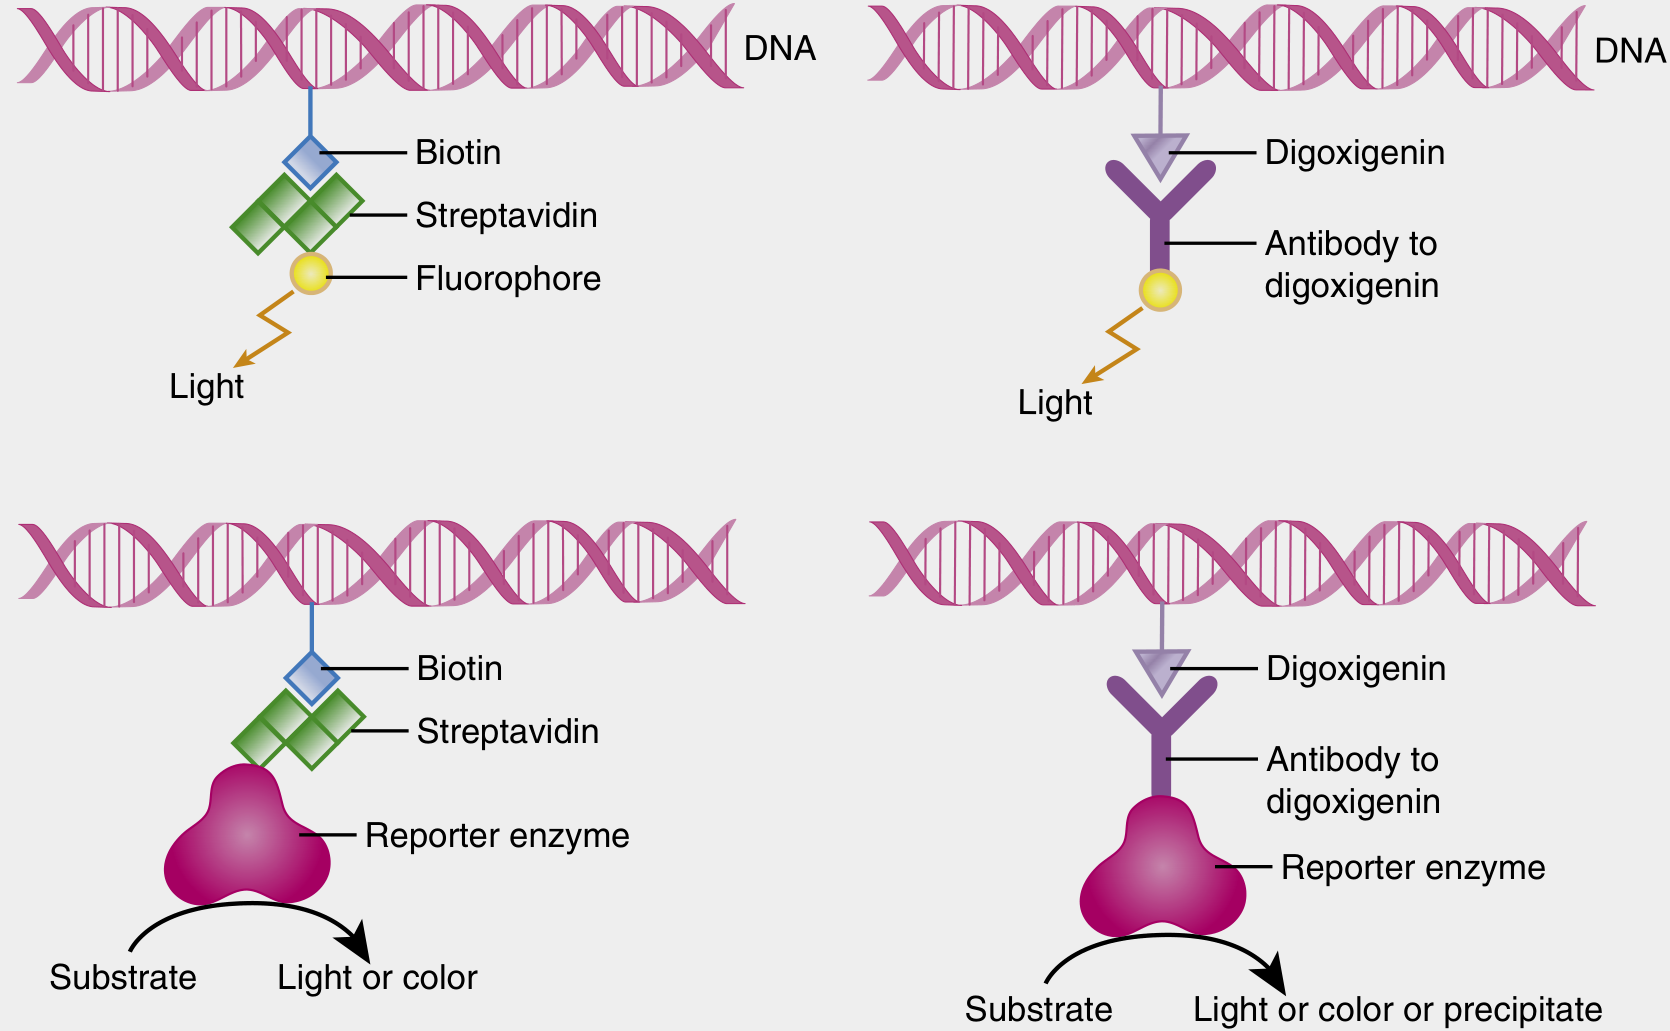
\includegraphics[width=0.7\linewidth]{../images/fluorescent_labelling} 

}

\caption{DNA can be synthesized in vitro with a uracil nucleotide linked to biotin or digoxigenin. Streptavidin binds tightly to avidin (left panels), and antibody to digoxigenin binds to digoxigenin (right panels). Streptavidin and antibody to digoxigenin can be conjugated to a fluorophore that emits light of specific wavelengths (top panels) or to reporter enzymes such as horseradish peroxidase or alkaline phosphatase (lower panels). Reporter enzymes act on different substrates, some of which release light and others that form a colored precipitate.}\label{fig:fluorescent-tags}
\end{figure}
\end{frame}

\begin{frame}{FISH technique}
\protect\hypertarget{fish-technique}{}
\begin{itemize}
\tightlist
\item
  A method for detecting the presence of particular genes (e.g., in a
  biological sample, in its native form), making use of DNA probe.
\item
  When those DNA probes hybridize to each of their respective particular
  genes of biological sample (i.e., that they were selected to be
  complementary to), each DNA probe's ``tag'' fluoresces at a different
  wavelength (different ``color''), thereby indicating positively the
  presence in sample of that particular gene.
\end{itemize}
\end{frame}

\begin{frame}{}
\protect\hypertarget{section-4}{}
\begin{itemize}
\tightlist
\item
  For example, if the color of the band is red it represents the base
  `T,' because the dideoxy Thyamidine Triphosphate (ddTTP) is labeled
  with a red dye. Similarly, yellow is for `G,' green is for `A,' and
  blue represents the base `C.'
\item
  In fluorescence \emph{in situ} hybridization (FISH), the
  clone\footnote[frame]{A probe may also be called a clone of a gene because it is designed such that it complementarily hybridizes with the gene}
  is labeled with a fluorescent dye (digoxigenin and / or biotin), and a
  partially denatured chromosome preparation is bathed in the probe.
\end{itemize}
\end{frame}

\begin{frame}{}
\protect\hypertarget{section-5}{}
\begin{itemize}
\tightlist
\item
  The probe binds to the chromosome in situ, and the location of the
  cloned fragment is revealed by a bright fluorescent spot when looked
  under UV illumination.
\item
  An extension of FISH is chromosome painting or multicolor \emph{in
  situ} hybridization.
\item
  Sets of cloned DNA known to be from specific chromosomes or specific
  chromosome regions are labeled with different fluorescent dyes.
\item
  These dyes then ``paint'' specific regions and identify them under the
  microscope. If a clone of a gene of unknown location is labeled with
  yet another dye, its position can be established in the painted array.
\end{itemize}
\end{frame}

\begin{frame}{}
\protect\hypertarget{section-6}{}
\begin{figure}
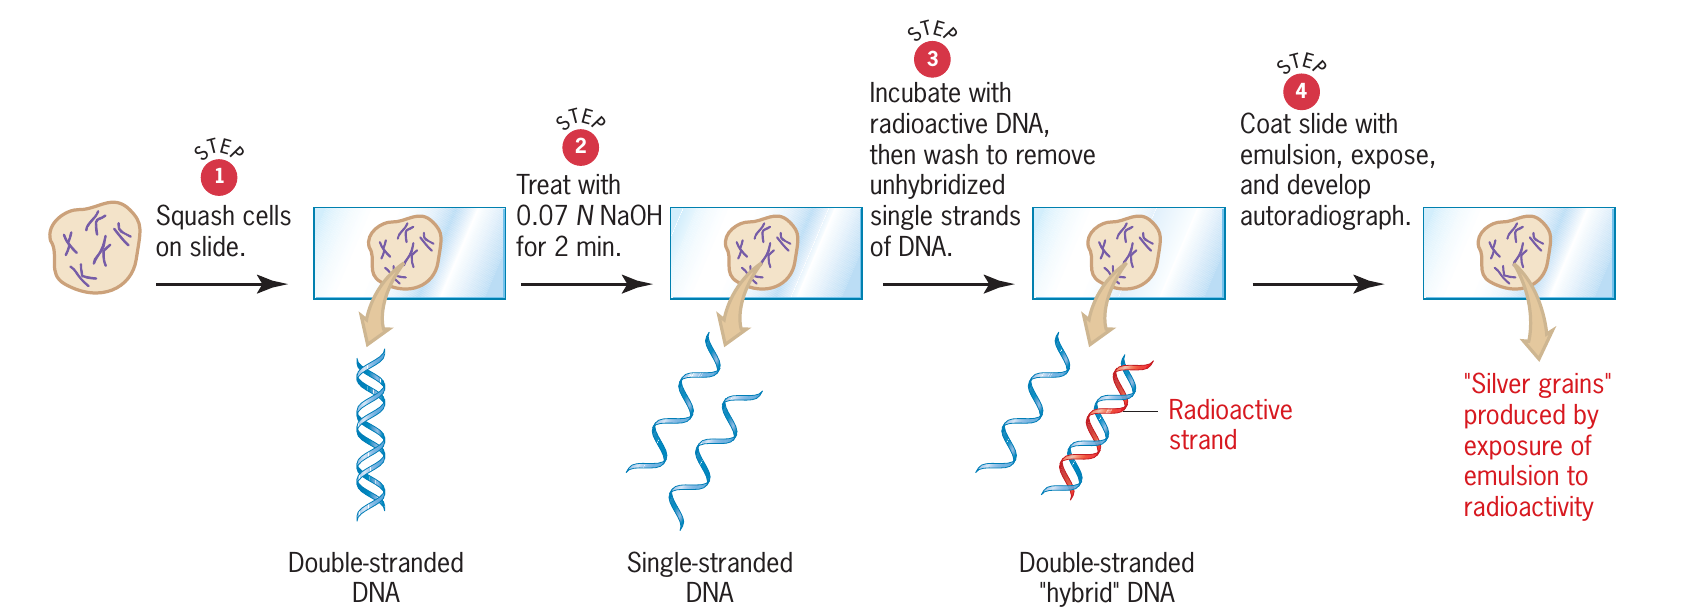
\includegraphics[width=0.7\linewidth]{./../images/insitu_hybrid_steps} \caption{Steps in in-situ hybridization}\label{fig:insitu-hybridization}
\end{figure}
\end{frame}

\hypertarget{isolation-of-dna}{%
\section{Isolation of DNA}\label{isolation-of-dna}}

\begin{frame}{}
\protect\hypertarget{section-7}{}
\begin{itemize}
\tightlist
\item
  Cell structure and organelles present a natural barrier.
\item
  Bacteria are easiest to manipulate because they have no cell wall or
  tissue barriers.
\item
  Distinction between two DNAs (genomic and mitochondrial) is made based
  on their sizes.
\item
  The first step in making recombinant DNA is to isolate donor and
  vector DNA.
\end{itemize}
\end{frame}

\begin{frame}{}
\protect\hypertarget{section-8}{}
\begin{itemize}
\tightlist
\item
  The procedure used for obtaining vector DNA depends on the nature of
  the vector.
\item
  Bacterial plasmids are commonly used vectors, and these plasmids must
  be purified away from the bacterial genomic DNA. A protocol for
  extracting plasmid DNA by ultracentrifugation is summarized:

  \begin{itemize}
  \tightlist
  \item
    Plasmid DNA forms a distinct band after ultracentrifugation in a
    cesium chloride density gradient containing ethidium bromide.
  \item
    The plasmid band is collected by punching a hole in the plastic
    centrifuge tube.
  \item
    Another protocol relies on the observation that, at a specific
    alkaline pH, bacterial genomic DNA denatures but plasmids do not.
  \item
    Subsequent neutralization precipitates the genomic DNA, but plasmids
    stay in solution.
  \end{itemize}
\item
  Phages such as \(\lambda\) also can be used as vectors for cloning DNA
  in bacterial systems. Phage DNA is isolated from a pure suspension of
  phages recovered from a phage lysate.
\end{itemize}
\end{frame}

\begin{frame}{Isolation of nuclear DNA: Steps}
\protect\hypertarget{isolation-of-nuclear-dna-steps}{}
\begin{enumerate}
\tightlist
\item
  Tissue should be thin and soft to be useable. If such it should be
  powdered in liquid nitrogen with mortar and pestle. The powder is then
  transferred to centrifuge tube. In bacteria, lysozyme digestion
  degrades the peptidoglycan layer.
\item
  Then the extraction buffer is added
  (CTAB\footnote[frame]{Cetyltrimethyl ammonium bromide is a surfactant useful for isolation of DNA from tissues containing high amounts of polysaccharides.}
  and sodium dodecyl sulfate (SDS, a detergent) buffer is widely used in
  plants) and mixed well. Then incubate at \(60^\circ C\) for one hour
  in a water bath.
\item
  Now centrifuge the solution and remove the precipitate, and transfer
  the supernatant (liquid) to another centrifuge tube. In animals,
  separation of intracellular components from the insoluble remains
  (cellular membranes, bones, cartilage, etc.) is done by either
  centrifugation or chemical extraction.
\end{enumerate}
\end{frame}

\begin{frame}{}
\protect\hypertarget{section-9}{}
\begin{enumerate}
\setcounter{enumi}{3}
\tightlist
\item
  Extract this solution with chloroform-isoamyl alcohol. All the organic
  and lipids will separate to the phenol-chloroform layer and DNA will
  be in the aqueous layer (stays above). Take the aqueous layer and
  again extract it with phenol-chloroform and repeat the step, if
  necessary.
\end{enumerate}

\begin{itemize}
\tightlist
\item
  This method of separating components using chemical extraction uses
  the properties of phenol to remove unwanted proteins from the DNA.
  phenol-chloroform (augmented with isoamyl alcohol) that dissolves 60\%
  to 70\% of all living matter, especially proteins.
\item
  Enzyme ribonuclease (RNase) will digest RNA into ribonucleotides.
\item
  If the mixture is acidic, DNA will precipitate into the organic phase
  while RNA remains in the aqueous phase because DNA is more readily
  neutralized than RNA.
\end{itemize}

\begin{enumerate}
\setcounter{enumi}{4}
\tightlist
\item
  Finally, the aqueous layer containing DNA is precipitated with
  ice-cold isopropanol or ethyl alcohol. The DNA should appear as white
  or creamy strands or fibers and can be separated or taken out with a
  glass rod.
\end{enumerate}

\begin{itemize}
\tightlist
\item
  Thus obtained DNA can be dissolved in Tris EDTA buffer for storage.
\end{itemize}
\end{frame}

\hypertarget{restriction-enzymes-restrictase-endonuclease-restriction-endonucleases}{%
\section{Restriction enzymes (Restrictase, Endonuclease, Restriction
endonucleases)}\label{restriction-enzymes-restrictase-endonuclease-restriction-endonucleases}}

\begin{frame}{}
\protect\hypertarget{section-10}{}
\begin{itemize}
\tightlist
\item
  Bacterial DNA cleaving enzymes recognize short sequence and are able
  to make double stranded cuts.
\item
  Function:

  \begin{itemize}
  \tightlist
  \item
    Destroy foreign DNA: Restrictase in the original bacterium cuts
    foreign DNA at several sites along the enemy foreign DNA molecule.
  \end{itemize}
\item
  Particular restrictase recognizes only one type of DNA sequence.
\item
  For example: EcoRI is a restrictase isolated from Escherichia coli.
\item
  Its palindrome sequence is: 5'GAATTC 3' //3'CTTAAG 5'.
\end{itemize}
\end{frame}

\begin{frame}{}
\protect\hypertarget{section-11}{}
\begin{itemize}
\tightlist
\item
  There are points of symmetry between the bases AT and TA in the
  palindrome and cutting site of the restrictase is away from the point
  of symmetry.
\item
  The EcoRI cuts between GA and AG in the palindromes.
\item
  The Eco RI is six base-cutter enzyme or nuclease and it produces
  staggered and sticky ends.
\item
  Some restrictases cut at the point of symmetry and produces blunt
  ends.
\item
  DNA joins can be made through blunt end cuts too.
\item
  A particular restrictase always recognizes unique base sequence
  whatever may be the source of the DNA.
\end{itemize}
\end{frame}

\begin{frame}{}
\protect\hypertarget{section-12}{}
\begin{figure}
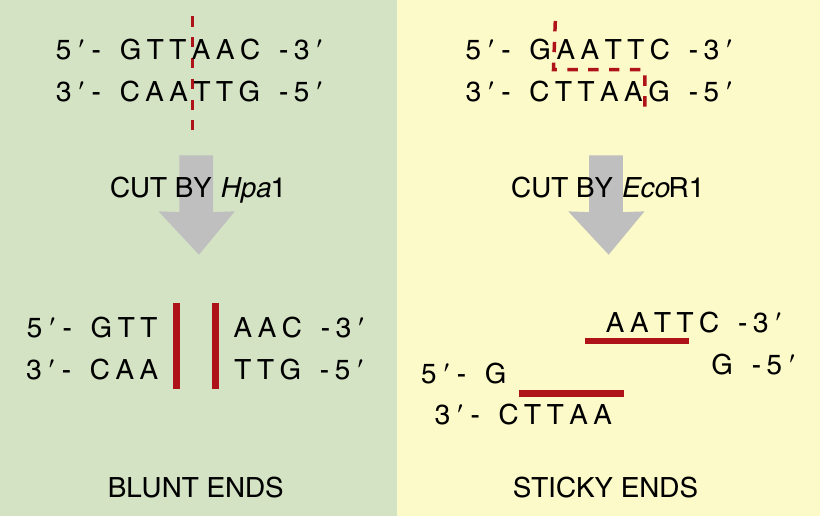
\includegraphics[width=0.55\linewidth]{./../images/restriction_enzymes} \caption{Mode of action of common restriction enzymes.}\label{fig:restriction-enzymes}
\end{figure}
\end{frame}

\begin{frame}{}
\protect\hypertarget{section-13}{}
\begin{itemize}
\tightlist
\item
  Restriction fragments of DNA molecules, produced by the same enzyme
  from the same or different sources contain identical staggered cut
  ends.
\item
  Since these ends can overlap and complementary base pairing can occur,
  fragments from different sources may join together to form hybrid
  molecules.
\item
  If the joined DNA fragments are treated with DNA ligase, they will be
  permanently joined together.
\end{itemize}
\end{frame}

\begin{frame}{}
\protect\hypertarget{section-14}{}
\begin{figure}
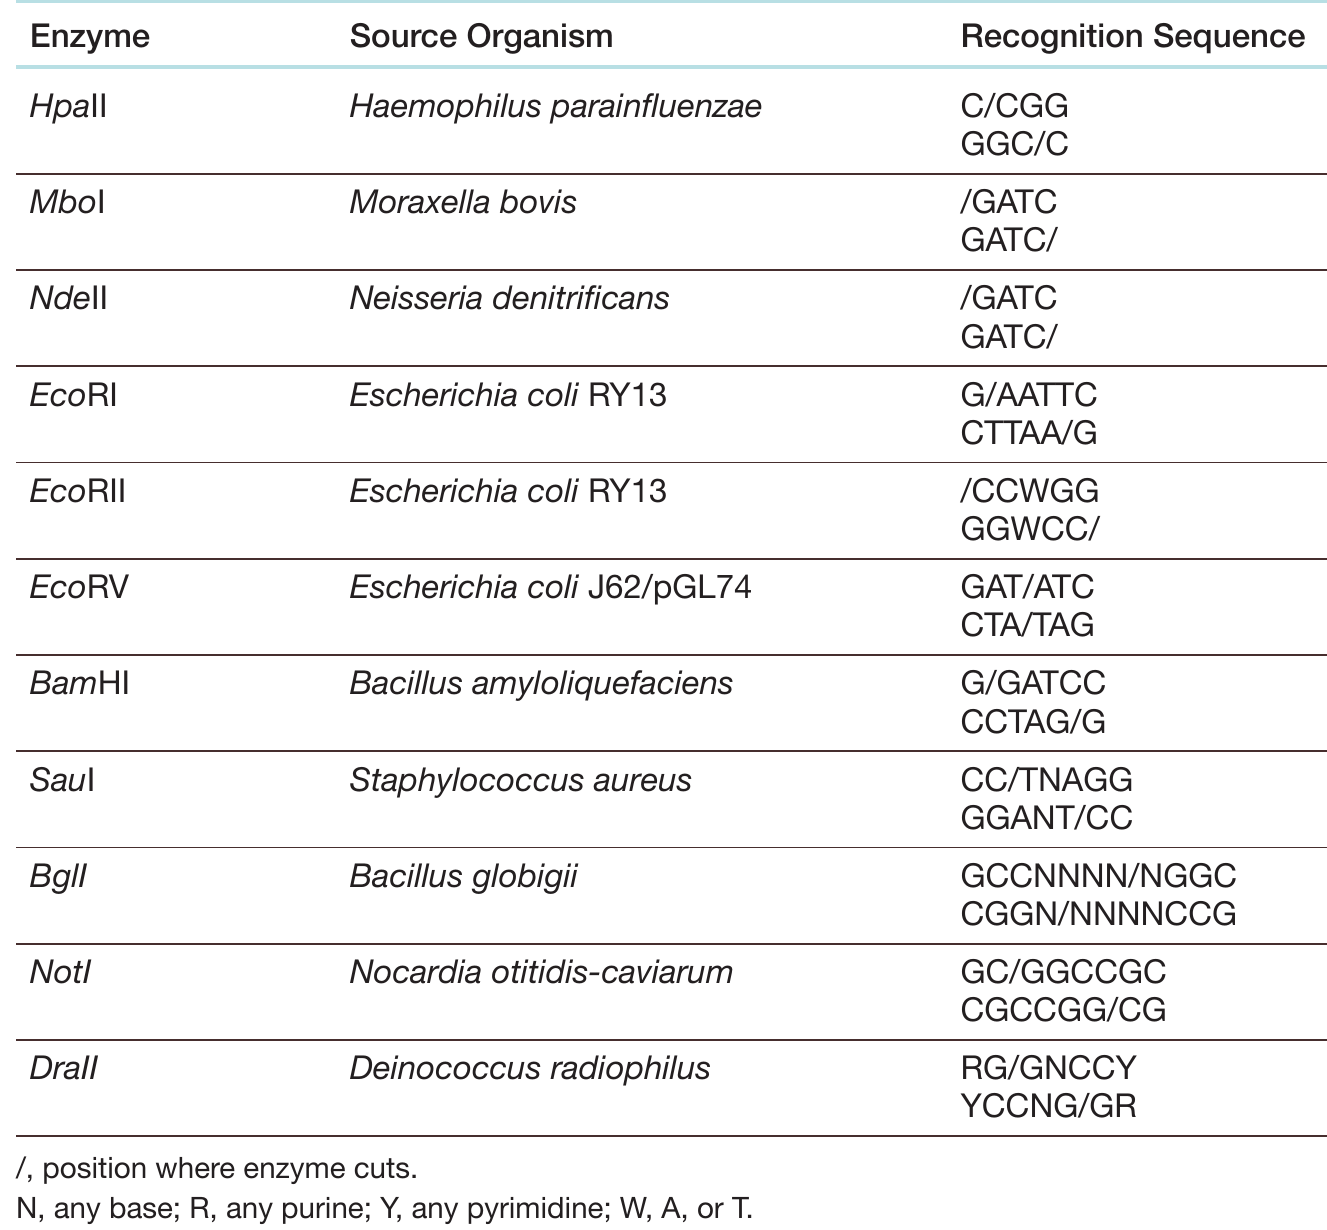
\includegraphics[width=0.54\linewidth]{./../images/restriction_enzymes_ex} \caption{Common restriction enzymes}\label{fig:restriction-enzymes-ex}
\end{figure}
\end{frame}

\begin{frame}{}
\protect\hypertarget{section-15}{}
\begin{itemize}
\item
  Restriction enzymes have been exploited to cut DNA at specific sites,
  since each restriction enzyme has a particular recognition sequence.
  Difference in cleavage site determine the type of restriction enzyme.

  \begin{itemize}
  \tightlist
  \item
    Type I restriction enzymes cut the DNA strand 1000 or more base
    pairs from the recognition sequence.
  \item
    Type II restriction enzymes cut in the middle of the recognition
    sequence and are the most useful in genetic engineering. The Type II
    restriction enzymes can form \emph{both} sticky or \emph{blunt}
    ends.
  \end{itemize}
\item
  The recognition sequences of Type II restriction enzymes are usually
  inverted repeats so that the enzymes cut between the same bases on the
  both strands.
\end{itemize}
\end{frame}

\hypertarget{formation-of-recombinant-dna}{%
\section{Formation of recombinant
DNA}\label{formation-of-recombinant-dna}}

\begin{frame}{Constructing rDNA: steps}
\protect\hypertarget{constructing-rdna-steps}{}
\begin{enumerate}
\tightlist
\item
  Digest the vector DNA with a suitable restriction endonuclease and
  make it linear with or without sticky ends, which is determined by the
  type of RE used.
\item
  Next, isolate the DNA fragment carrying the gene by digesting the
  genome or the source DNA strand with the sam eRE used for cutting the
  vector.
\item
  Incubate the linearized vector and the target DNA cut with the same
  restriction enzyme in the presence of DNA ligase. During this process,
  the sticky ends of the two DNA strands come closer by the base
  complementation and become hydrogen bonded to each other.
\item
  The result is the formation of recombinant DNA molecule of vector and
  the target DNA or insert DNA -- the combination is called a
  \textbf{construct}.
\item
  Sometimes double digestion of vector and foreign DNA inserts is done
  by two restriction enzymes to prevent re-annealing to some extent.
\end{enumerate}
\end{frame}

\begin{frame}{}
\protect\hypertarget{section-16}{}
\begin{figure}
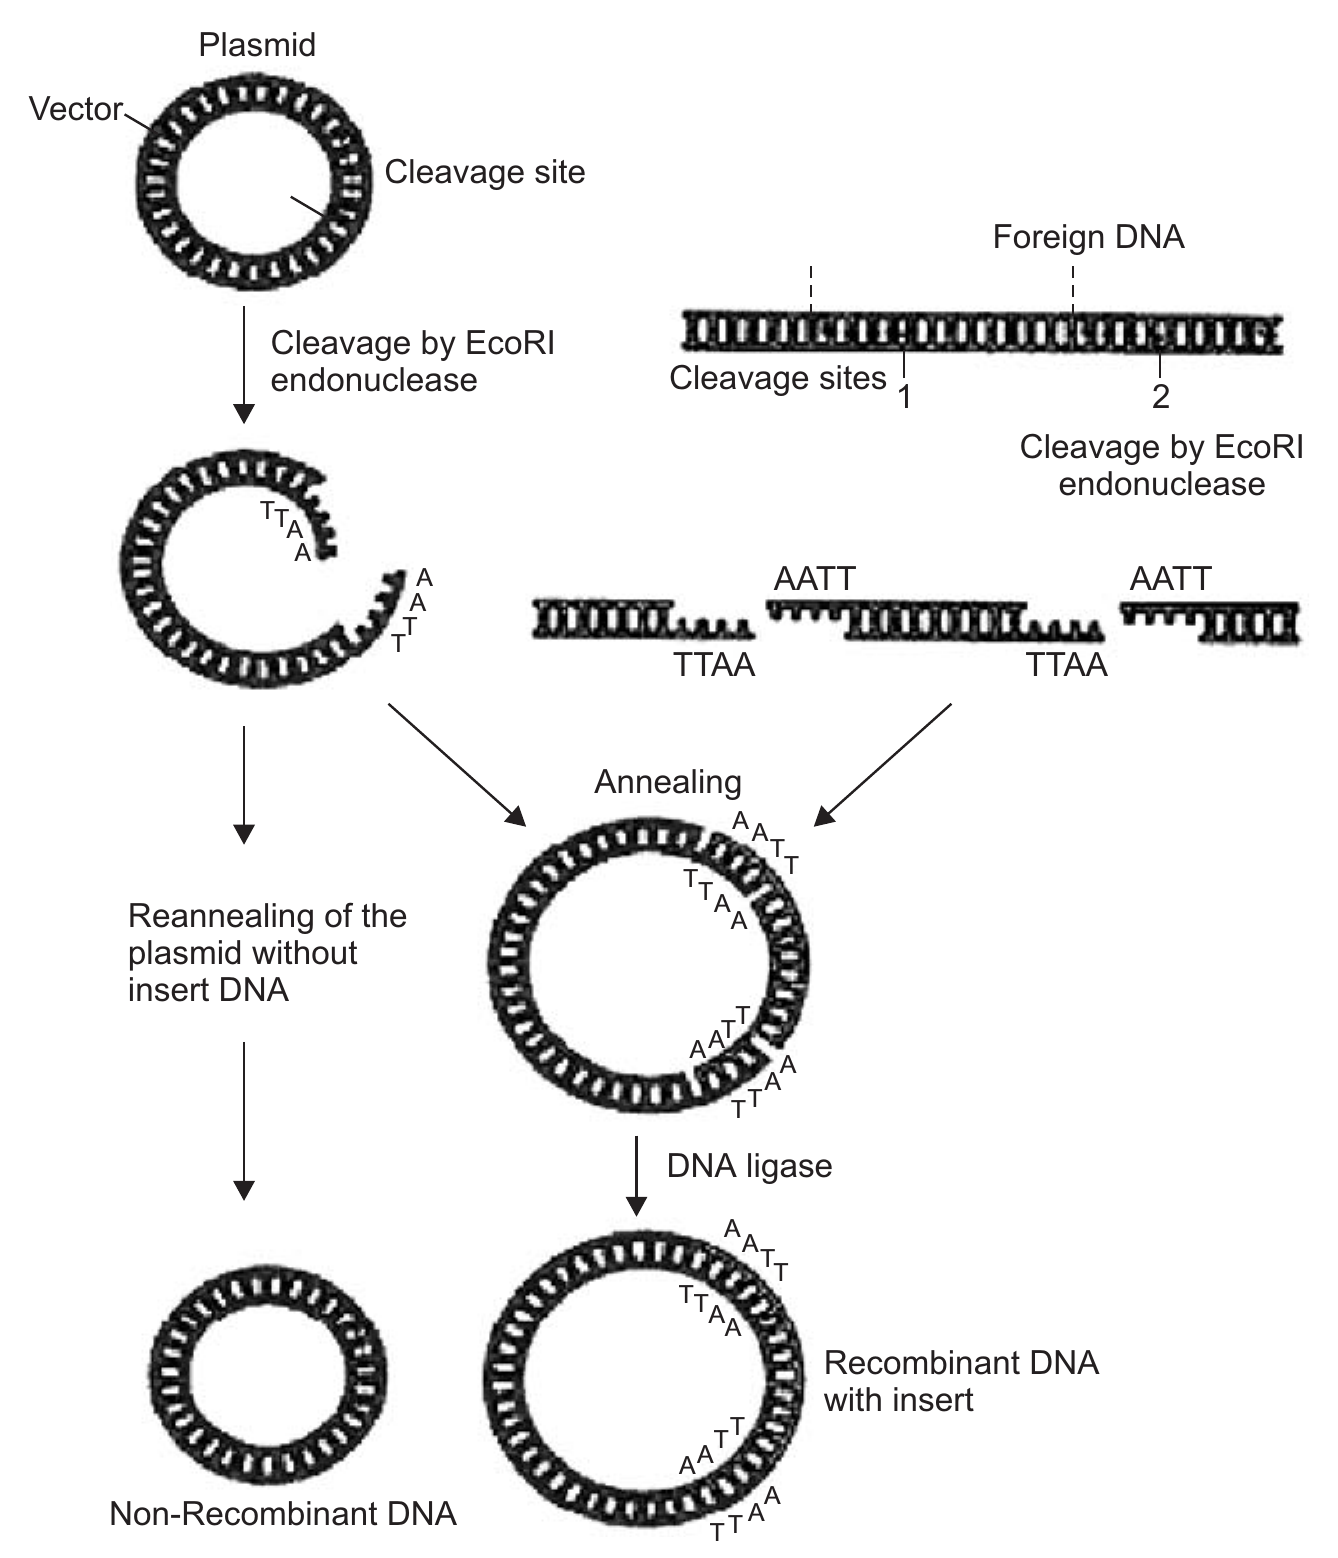
\includegraphics[width=0.4\linewidth]{./../images/construction_rdna_molecule} \caption{A general strategy for construction of rDNA molecule}\label{fig:rdna-construction}
\end{figure}
\end{frame}

\hypertarget{vectors}{%
\section{Vectors}\label{vectors}}

\begin{frame}{}
\protect\hypertarget{section-17}{}
\begin{itemize}
\tightlist
\item
  In in vivo replication of DNA, an investigator begins with a sample of
  DNA molecules containing the gene of interest (called donor DNA).
\item
  Fragments of the donor DNA are inserted into a specially designed
  plasmid or bacterial virus that will ``carry'' and amplify the gene of
  interest and hence called \textbf{vectors}.
\item
  First, the donor DNA molecules are cut up by using ``molecular
  scissors'' into manageable sizes of fragments.
\item
  Next, each fragment is inserted into a cut vector chromosome to form
  recombinant DNA molecules. The recombinant DNA molecules are
  transferred into bacterial cells, and, generally, only one recombinant
  molecule is taken up by each cell. Within each bacterial cell, the
  recombinant molecule is amplified along with the vector during cell
  division.
\item
  From a single cell, this process results in a clone of identical
  cells, each containing the recombinant DNA molecule, and so this
  technique of amplification is called \textbf{DNA cloning}.
\end{itemize}
\end{frame}

\begin{frame}{}
\protect\hypertarget{section-18}{}
\begin{itemize}
\tightlist
\item
  Suitability as a cloning vector:

  \begin{itemize}
  \tightlist
  \item
    Small molecule for manipulation,
  \item
    Prolific replication,
  \item
    Amplification of inserted DNA-plasmid
  \item
    Must contain few convenient restriction sites (aka polylinker
    sites).
  \item
    Way to identify and recover the desired recombinant molecule
  \end{itemize}
\item
  They are mostly plasmids, viral vectors (\(\lambda\) phage; single
  stranded phages), cosmids and expression vectors.
\end{itemize}
\end{frame}

\begin{frame}{Plasmids}
\protect\hypertarget{plasmids}{}
\begin{itemize}
\tightlist
\item
  They are smaller circular DNA molecules - distinct from the main
  bacterial chromosome. They replicate independently.
\item
  Plasmids are replicons that are stably inherited in extrachromosomal
  state.
\item
  They do get elliminated but at a very low rate, typically 1 per every
  \(10^{7}\) cells.
\item
  When a plasid is capable of integrating into bacterial chromosome it
  is called \textbf{episome} (but it is a broader term).
\item
  Plasmids carry genes that confer advantages on their host cell at
  certain conditions. Most but not all plasmids are dispensable.
\item
  The host cell in return provides conditions necessary for limited
  replication of the plasmid, and its transmission to daughter cells
  whenever the cell divides, thus allowing the plasmid to permeate in
  bacterial population.
\end{itemize}
\end{frame}

\begin{frame}{}
\protect\hypertarget{section-19}{}
\begin{itemize}
\tightlist
\item
  Plasmids have variable sizes, viz.~starting with only 3 genes to
  several hundreds of those. And a single bacterial cell may contain
  zero or more plasmids (upto 11).
\item
  Plasmids constantly evolve.
\item
  Recombination and host integration of plasmids is generally mediated
  by transposable genetic elements.
\item
  Plasmid vectors are generally genetically engineered to contain a
  number of restriction sites (\emph{polylinker} or \emph{multiple
  cloning site}) for commonly used restriction enzymes in a region.
\end{itemize}
\end{frame}

\begin{frame}{Plasmid types}
\protect\hypertarget{plasmid-types}{}
\begin{itemize}
\tightlist
\item
  F plasmids: Responsible for bacterial conjugation; carry genes for the
  development of F pili and for conjugation. Are conjugative plasmids.
\item
  R plasmids: Carry genes for resistance to antibiotics and
  antibacterial drugs; aka Resistance Transfer Factor (RTF).
\item
  Col plasmids: Code for colicins (proteins that kill sensitive \emph{E.
  coli} cells). Are mostly non conjugative.
\end{itemize}
\end{frame}

\begin{frame}{Plasmids used in rDNA}
\protect\hypertarget{plasmids-used-in-rdna}{}
\begin{itemize}
\tightlist
\item
  Plasmids are easily isolated in large numbers from bacterial cells,
  and usually have a small limited number of restriction sites.
\item
  Plasmids with drug-resistance genes provide a convenient way to select
  for potentially transformed bacterial cells (Not all transformed cells
  might contain gene of interest).
\item
  It is desirable to be able to identify bacterial colonies with
  plasmids containing DNA inserts. Such a feature is part of the pUC18
  plasmid vector.
\item
  DNA inserts disrupt a gene (lacZ) in the plasmid that encodes an
  enzyme (\(\beta\)-galactosidase) necessary to cleave a compound added
  to the petri plate agar (X-gal). Thus, the colonies that contain the
  plasmids with the DNA insert will be white rather than blue (they
  cannot cleave X-gal because they do not produce
  \(\beta\)-galactosidase)
\end{itemize}

(Refer to Chapter 20 of Klug et al. (2019) for details of
\textbf{Blue-White screening})
\end{frame}

\begin{frame}{}
\protect\hypertarget{section-20}{}
\begin{figure}
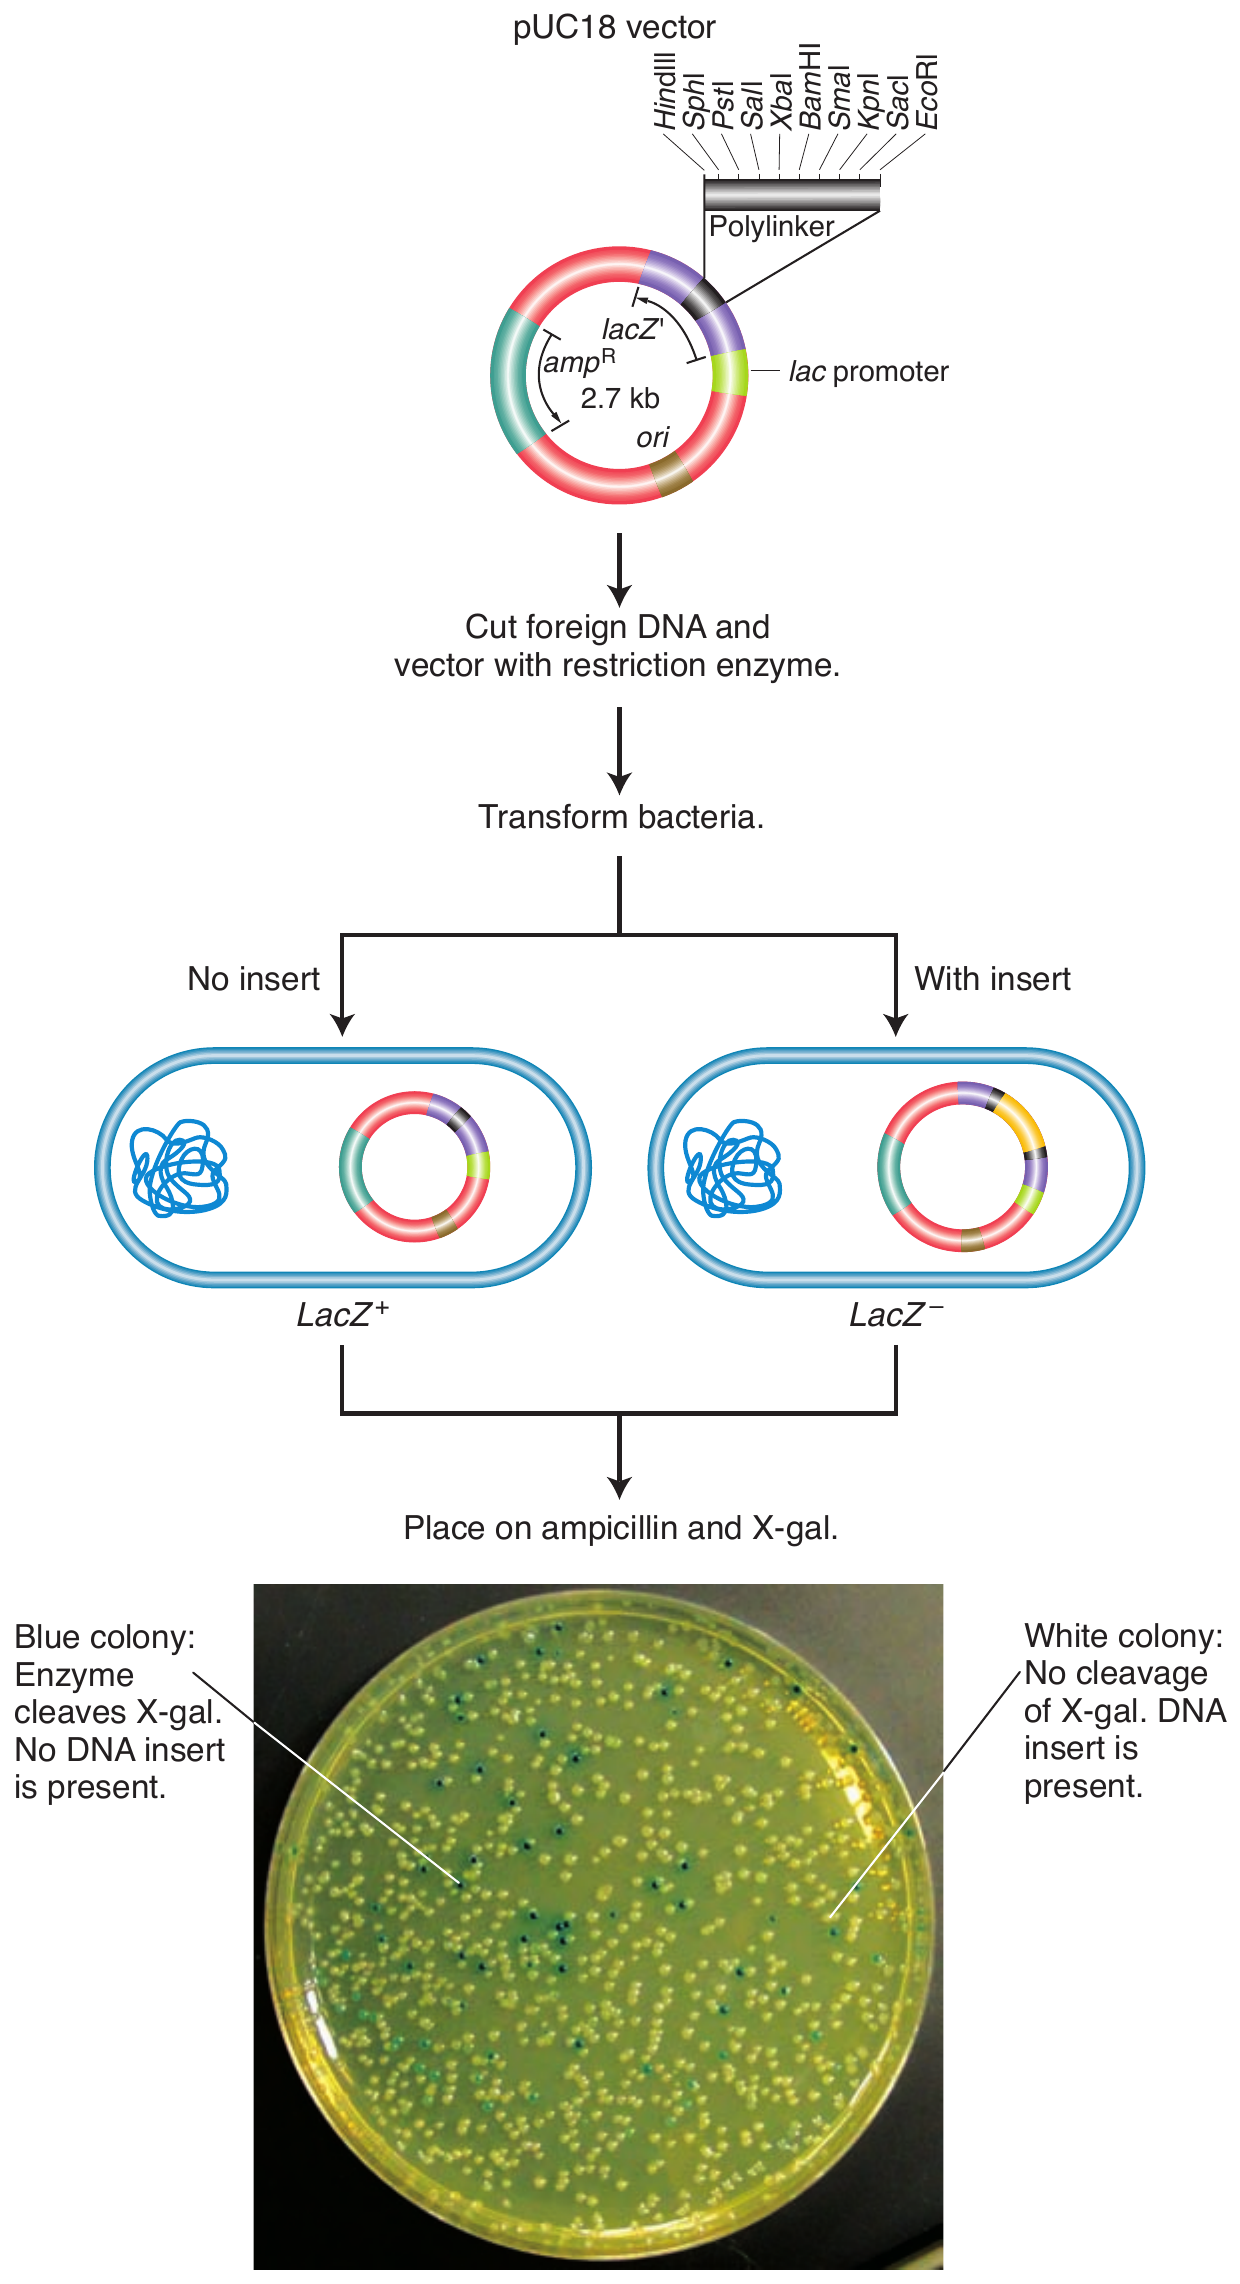
\includegraphics[width=0.28\linewidth]{./../images/plasmid_vector_pUC18} \caption{Use of plasmid vector, pUC18}\label{fig:phage-vector}
\end{figure}
\end{frame}

\begin{frame}{Viral vectors}
\protect\hypertarget{viral-vectors}{}
\begin{itemize}
\tightlist
\item
  Virus infects host cells with high efficiency.
\item
  The cloned genes can be introduced into cells at a significantly
  higher frequency than by simple transformation.
\item
  Some viral vectors are specialized for producing high levels of
  proteins by the cloned genes. Viral vectors are vehicles of choice for
  gene-therapy.
\item
  A \textbf{bacteriophage} vector harbors DNA as an insert ``packaged''
  inside the phage particle. Different classes of bacteriophage vectors
  can carry different sizes of donor DNA insert. Bacteriophage
  \(\lambda\) is an effective cloning vector for double-stranded DNA
  inserts as long as 45 kb (more than twice that of plasmid vectors).
  The central part of the phage genome is not required for replication
  or packaging of \(\lambda\) DNA molecules in E. coli and so can be cut
  out by restriction enzymes and discarded. The deleted central part is
  then replaced by inserts of donor DNA.
\item
  As \(lambda\) phase replicate inside the bacterial host cells, they
  lyse and form the clear spots known as plaques on the bacterial lawn.
\end{itemize}
\end{frame}

\begin{frame}{Bacterial artificial chromosomes (BACs) and Yeast
artificial chromosomes (YACs)}
\protect\hypertarget{bacterial-artificial-chromosomes-bacs-and-yeast-artificial-chromosomes-yacs}{}
\begin{itemize}
\tightlist
\item
  Useful for cloning large fragments of DNA -- for study such as mapping
  and analysis of large eukaryotic genome.
\item
  Although large and can accept DNA inserts in the range of 100-300 kb,
  BACs are low copy number plasmids (only 1 or 2 per bacterial cell).
\item
  YACs have telomeres at each end, \emph{ori} sites and a centromere
  (much like a chromosome).
\item
  They can clone DNA inserts from 100-1000 kb and are currently more
  popular as expression vectors due to being able to express eukaryotic
  genes requiring post-transcriptional modification of proteins.
\end{itemize}
\end{frame}

\begin{frame}{Constructing an YAC}
\protect\hypertarget{constructing-an-yac}{}
\scriptsize

\begin{itemize}
\tightlist
\item
  A YAC is built using an initial circular DNA plasmid, which is
  typically cut into a linear DNA molecule using restriction enzymes;
  DNA ligase is then used to ligate a DNA sequence or gene of interest
  into the linearized DNA, forming a single large, circular piece of
  DNA. The basic generation of linear yeast artificial chromosomes can
  be broken down into 6 main steps:
\item
  Ligation of selectable marker into plasmid vector: this allows for the
  differential selection of colonies with, or without the marker gene.
  An antibiotic resistance gene allows the YAC vector to be amplified
  and selected for in E. coli by rescuing the ability of mutant E. coli
  to synthesize leucine in the presence of the necessary components
  within the growth medium. TRP1 and URA3 genes are other selectable
  markers. The YAC vector cloning site for foreign DNA is located within
  the SUP4 gene. This gene compensates for a mutation in the yeast host
  cell that causes the accumulation of red pigment. The host cells are
  normally red, and those transformed with YAC only, will form colorless
  colonies. Cloning of a foreign DNA fragment into the YAC causes
  insertional inactivation of the gene, restoring the red color.
  Therefore, the colonies that contain the foreign DNA fragment are red.
\item
  Ligation of necessary centromeric sequences for mitotic stability
\item
  Ligation of Autonomously Replicating Sequences (ARS) providing an
  origin of replication to undergo mitotic replication. This allows the
  plasmid to replicate extrachromosomally, but renders the plasmid
  highly mitotically unstable, and easily lost without the centromeric
  sequences.
\item
  Ligation of artificial telomeric sequences to convert circular plasmid
  into a linear piece of DNA
\item
  Insertion of DNA sequence to be amplified (up to 1000kb)
\item
  Transformation yeast colony
\end{itemize}
\end{frame}

\hypertarget{methods-of-cloning}{%
\section{Methods of cloning}\label{methods-of-cloning}}

\begin{frame}{}
\protect\hypertarget{section-21}{}
\begin{itemize}
\tightlist
\item
  The recombinant plasmid is introduced into a bacterial cell as in
  transformation.
\item
  This is easily done by adding the vector to bacterial cells in the
  presence of \(\mathrm{CaCl_2}\) or by using electroporation.
\item
  Once foreign DNA introgressed plasmid inters the bacterial cell, the
  plasmid is replicated (contain \emph{ori} sites) and the number
  increased.
\item
  The plasmid vector usually carries one or more antibiotic resistance
  markers so that when cultured on a medium containing the antibiotic,
  only bacterial cells containing the recombinant plasmid vector will
  survive and grow.
\item
  Each hybrid molecule results in a bacterial cell population with the
  same foreign DNA fragment being present in all the cells.
\item
  In this context, this piece of foreign DNA is referred to as being
  cloned. This constitutes the molecular cloning process.
\end{itemize}
\end{frame}

\begin{frame}{}
\protect\hypertarget{section-22}{}
\begin{itemize}
\tightlist
\item
  A major application of gene cloning is to have DNA fragments
  representing the entire genome of an organism cloned on plasmids. This
  constitutes a so-called gene library.
\item
  It represents a collection of plasmid containing fragments that is
  large enough so that each segment of the entire genomic DNA is
  represented at least once.
\item
  A general method for producing a gene library is called ``shotgun''
  cloning.
\item
  Clones of these plasmids are then maintained in the bacterial
  population.
\item
  Various techniques are available to probe the library for specific
  bacterial strains containing a fragment with a particular sequence.
\item
  One strategy involves the isolation of the mRNA transcript from tissue
  actively making large quantities of the protein whose gene is being
  sought.
\item
  This mRNA is radioactively labeled and reacted through Southern
  blotting with DNA isolated from the various library clones.
\item
  This isolated RNA will hybridize only to those clones carrying
  complementary DNA sequences.
\end{itemize}
\end{frame}

\begin{frame}{}
\protect\hypertarget{section-23}{}
\begin{itemize}
\tightlist
\item
  Another approach can be used to identify clones carrying specific
  genes. This is called cDNA cloning.
\item
  The mRNA transcript from the gene of interest can be isolated and a
  DNA copy of this RNA can be made with reverse transcriptase. This DNA
  is called copy DNA or cDNA.
\item
  The cDNA can be inserted into a plasmid and cloned in a bacterium.
  This cloned cDNA is used as the probe to identify library clones
  carrying that particular gene.
\item
  If the protein whose gene is sought is not present in large quantity,
  a small amount of the protein is purified, and the amino acid sequence
  of some portion of it is determined.
\item
  A piece of cDNA corresponding to this sequence can be synthesized.
\item
  This human made fragment is used as the probe for the clone of
  interest. Finally, if enough protein is produced to obtain antibodies,
  the various clones may be screened with antibody to identify clones in
  which the protein is being made.
\end{itemize}
\end{frame}

\hypertarget{related-concepts}{%
\section{Related concepts}\label{related-concepts}}

\begin{frame}{Restriction fragment length polymorphism}
\protect\hypertarget{restriction-fragment-length-polymorphism}{}
\begin{itemize}
\tightlist
\item
  First molecular marker technique that was applied on a larger scale.
\item
  When genotypes differ; then, their DNA sequences will be different,
  for instance, there will be mutations in restriction sites, or there
  may be insertions or deletion.
\item
  When the DNA of each genotype is cut with the same restriction enzyme,
  the resulting digests are separated on an electrophoresis gel, the DNA
  on the gel is transferred to a Southern blot, and the DNA on the blot
  is hybridized with a probe, differences in length of the hybridizing
  restriction fragments are visualized on the autoradiogram.
\end{itemize}
\end{frame}

\begin{frame}{}
\protect\hypertarget{section-24}{}
\begin{itemize}
\tightlist
\item
  Usually the probe allows detection of several alleles; there are,
  however, a few circumstances when just not all alleles present in the
  DNA can be observed, e.g.~when the fragment is very close to other
  fragments, the probe hybridizes that too.
\item
  In the latter case the probe is homologous to more than just one
  region on the genome (it is not a single copy probe). When not all
  alleles can be observed this leads to \textbf{dominant} marker
  genotypes.
\item
  For instance, a diploid individual having a single band can be of
  genotype AA, i.e.~it has two copies of the same band, or A\_, i.e., it
  has just one copy of the band with the other band being unobservable.
\end{itemize}
\end{frame}

\begin{frame}{}
\protect\hypertarget{section-25}{}
\begin{itemize}
\tightlist
\item
  An unobservable band is said to correspond to a so-called
  \textbf{null-allele}.
\item
  Dominant genotypes provide less information for linkage analysis than
  \textbf{codominant} genotypes because of the corresponding uncertainty
  of the underlying real genotypes.
\item
  In some applications of RFLP, use was made of probes consisting of
  repetitive sequences (e.g., a sequence of 15 nucleotides repeated in
  tandem 10 times) with which homologous sequences are present at many
  places in a genome; such probes were called \textbf{minisatellite}
  probes and the band patterns on the autoradiogram were called genetic
  fingerprints.
\end{itemize}
\end{frame}

\begin{frame}{}
\protect\hypertarget{section-26}{}
\begin{itemize}
\tightlist
\item
  Sometimes same restrictase does not produce equal length restriction
  fragments among the members of the same biological species. It is
  because the palindromic sequences may have mutated.
\item
  In this case the same restrictase in the next individual of the same
  species makes long restriction fragments. But the clone will hybridize
  the longer restriction fragment. This way there will be variation in
  the length of the hybridized restriction fragments. The variation is
  called RFLP or Restriction Fragment Length Polymorphism.
\item
  The presence or absence of the restriction site can be treated as two
  alleles that can be thought of as + and -- alleles.
\end{itemize}
\end{frame}

\begin{frame}{}
\protect\hypertarget{section-27}{}
\begin{itemize}
\tightlist
\item
  The presence of the (+) in some individuals in the population and the
  absence (-) in others generates a restriction fragment length
  polymorphism or RFLP.
\item
  Restriction fragment is the fragment of DNA cut by restrictase but
  restriction fragment length is not the length of the restriction
  fragment, it is the length of the hybridized fragment of the
  restriction fragments with probe DNA or RNA.
\item
  The length varies among the segregating individuals of population or
  among the individuals of a same species.
\end{itemize}
\end{frame}

\begin{frame}{}
\protect\hypertarget{section-28}{}
\begin{figure}
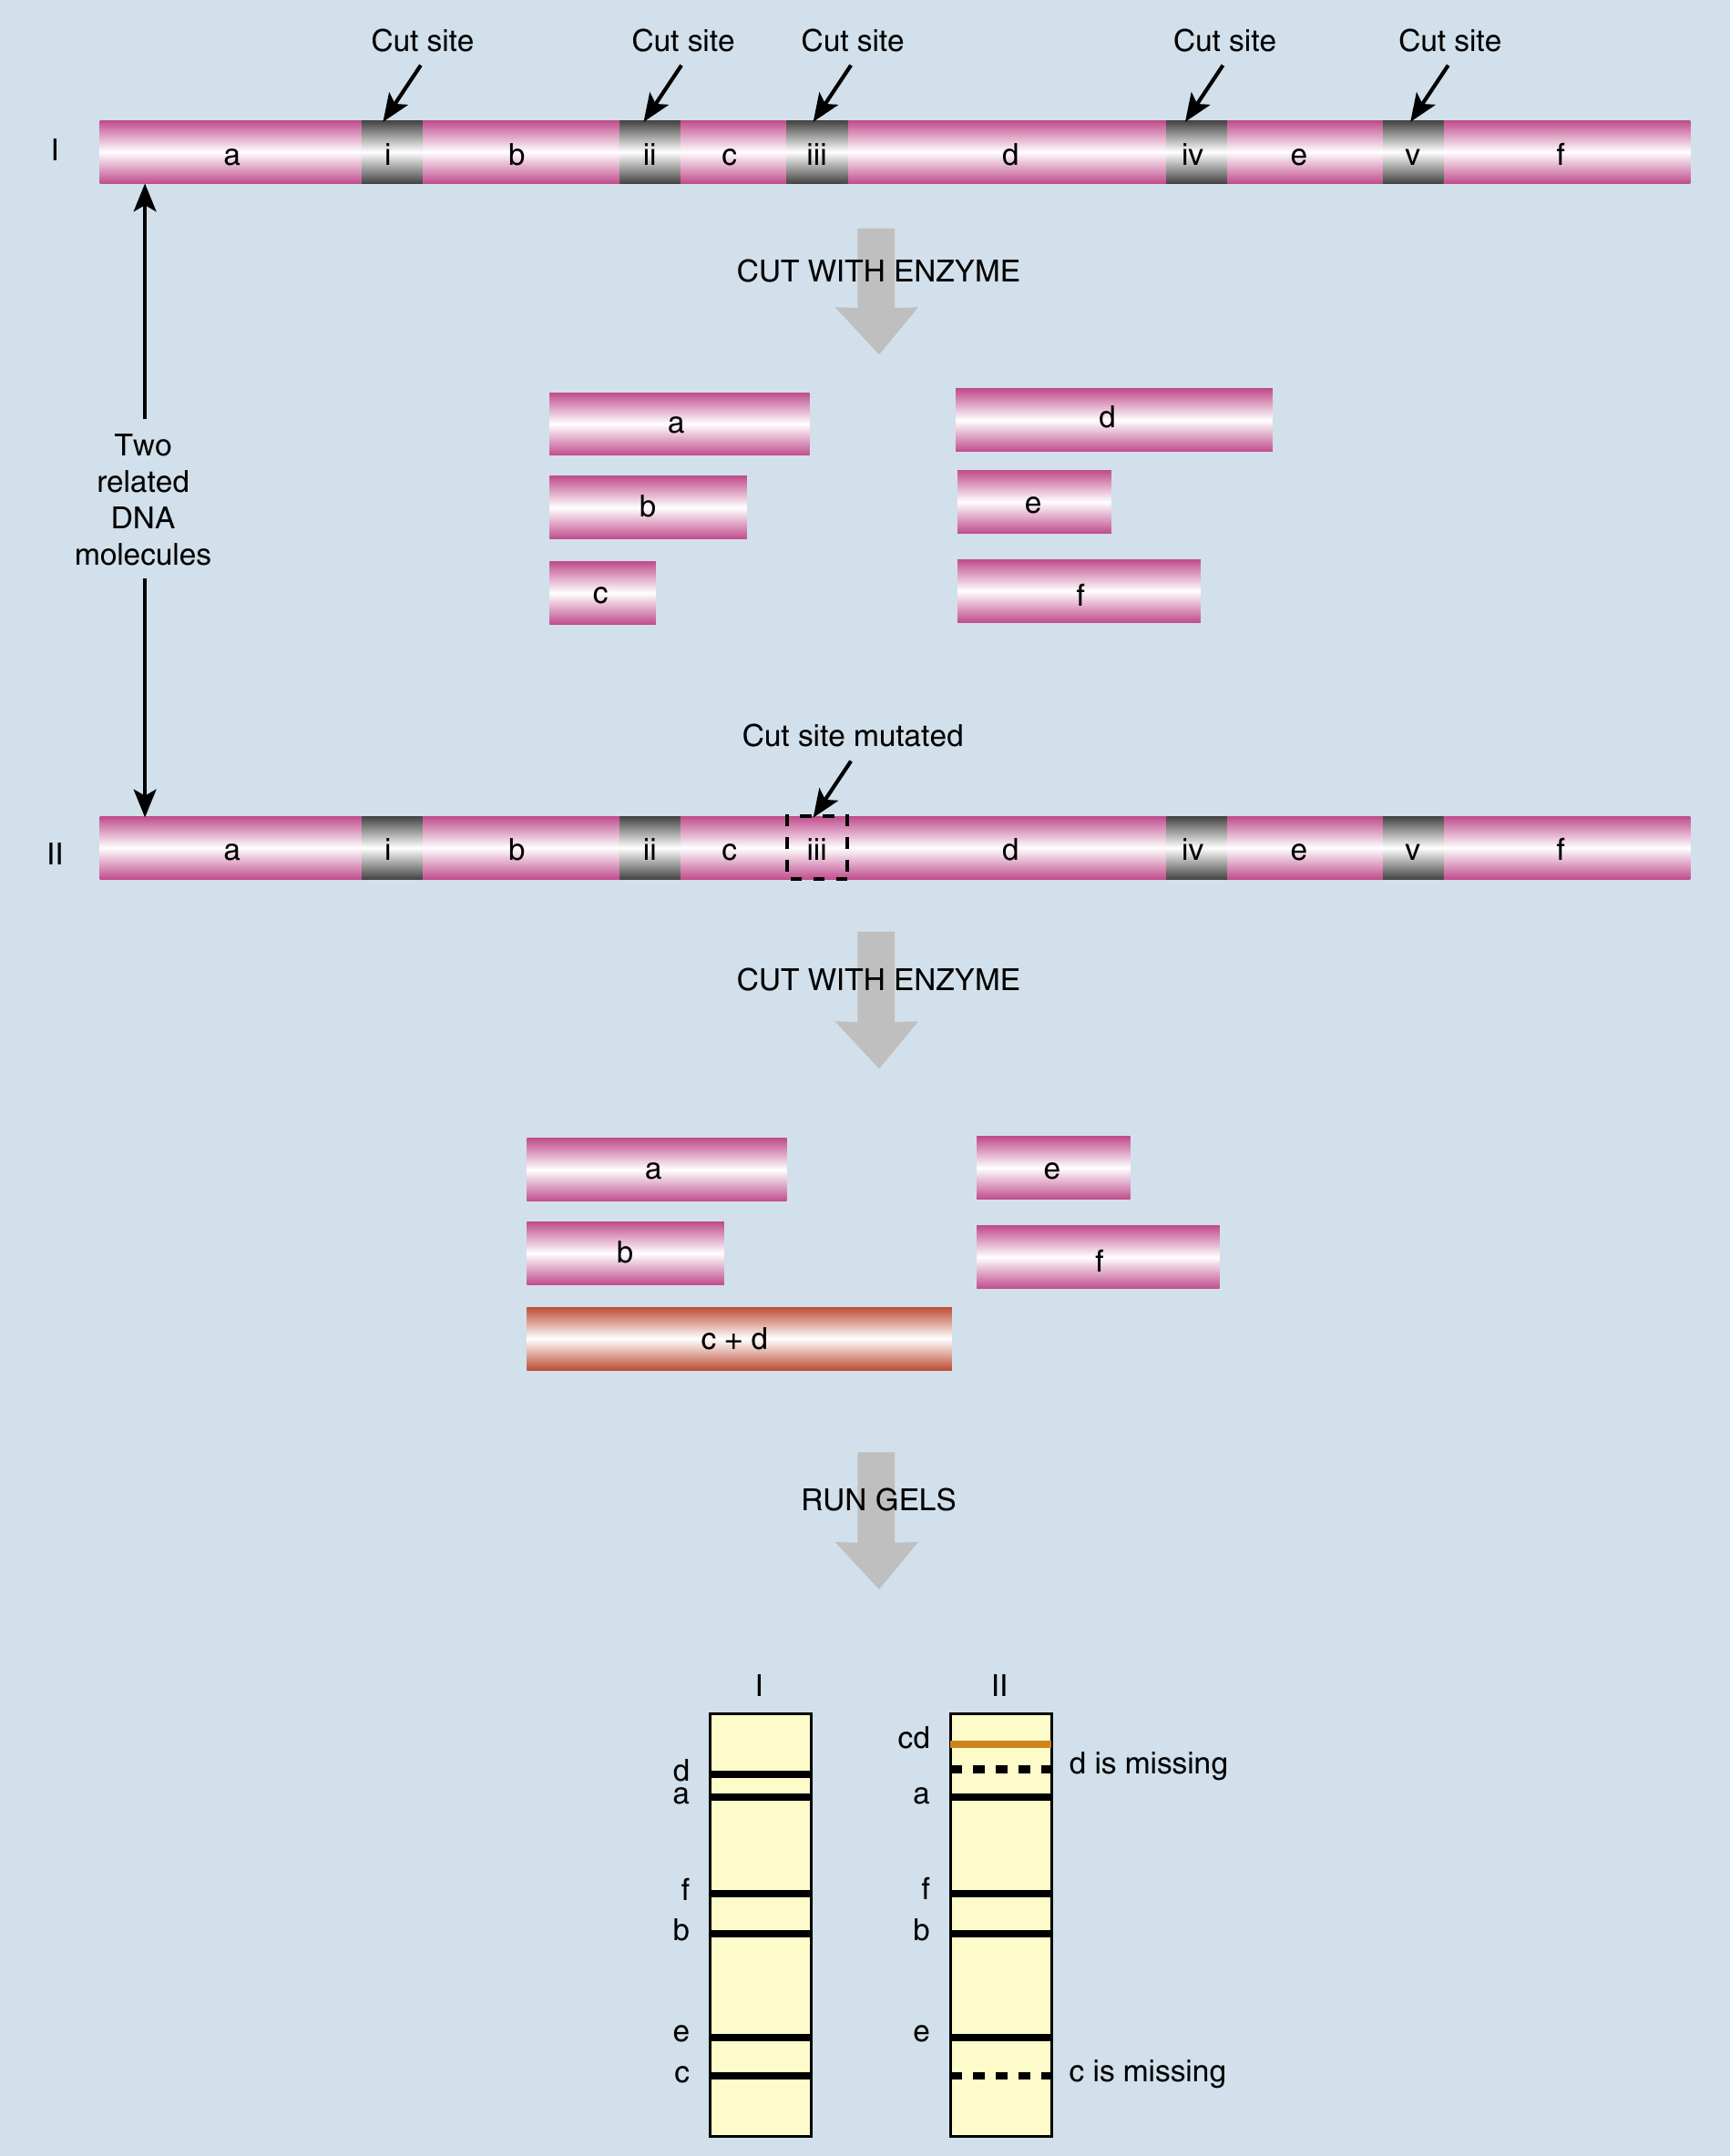
\includegraphics[width=0.35\linewidth]{./../images/rflp_analysis} \caption{DNA from related organisms shows small differences in sequence that cause changes in restriction sites. In the example shown, cutting a segment of DNA from the first organism yields six fragments of different sizes (labeled a–f on the gel). If the equivalent region of DNA from a related organism were digested with the same enzyme, a similar pattern would be expected. Here, a single-nucleotide difference is present, which eliminates one of the restriction sites. Consequently, digesting this DNA produces only five fragments. Fragments c and d are no longer seen but form a new band labeled cd.}\label{fig:rflp-analysis}
\end{figure}
\end{frame}

\begin{frame}{Southern blotting}
\protect\hypertarget{southern-blotting}{}
\begin{itemize}
\tightlist
\item
  In this technique, a DNA molecule is cut into discrete fragments by a
  restriction enzyme.
\item
  It is then electrophoresed through an agarose gel (fractionate). This
  separated the various fragments according to size.
\item
  This is called DNA fractionation.
\item
  The DNA is then denatured into single strands by exposing the gel to
  NaOH.
\item
  A few pieces of filter paper soaked in buffer are placed under the
  gel.
\item
  A large piece of nitrocellulose paper is layed over the agarose gel,
  followed by several layers of absorbent material such as filter paper.
\item
  This dry absorbent material pulls the buffer through the gel from the
  lower layer. This washes the DNA off the gel and onto the filter,
  where it covalently binds to the nitrocellulose filter.
\end{itemize}
\end{frame}

\begin{frame}{}
\protect\hypertarget{section-29}{}
\begin{itemize}
\tightlist
\item
  The positions of the DNA molecules on the filter are identical to
  their position in the gel.
\item
  The nitrocellulose filter containing the DNA is first dried and then
  exposed to a solution of 32P labeled mRNA from the gene to be
  isolated.
\item
  The radioactive mRNA hybridizes (hydrogen bonds) only with the
  single-stranded DNA in restriction fragments that contain
  complementary sequences.
\item
  The nitrocellulose filter is then removed and placed in contact with
  photographic film that when developed will reveal the fragments from
  the original gel containing complementary sequences to the mRNA used
  in the assay.
\item
  This procedure allows specific identification of restriction fragments
  containing DNA sequences to specific RNA molecules.
\end{itemize}
\end{frame}

\begin{frame}{}
\protect\hypertarget{section-30}{}
\begin{figure}
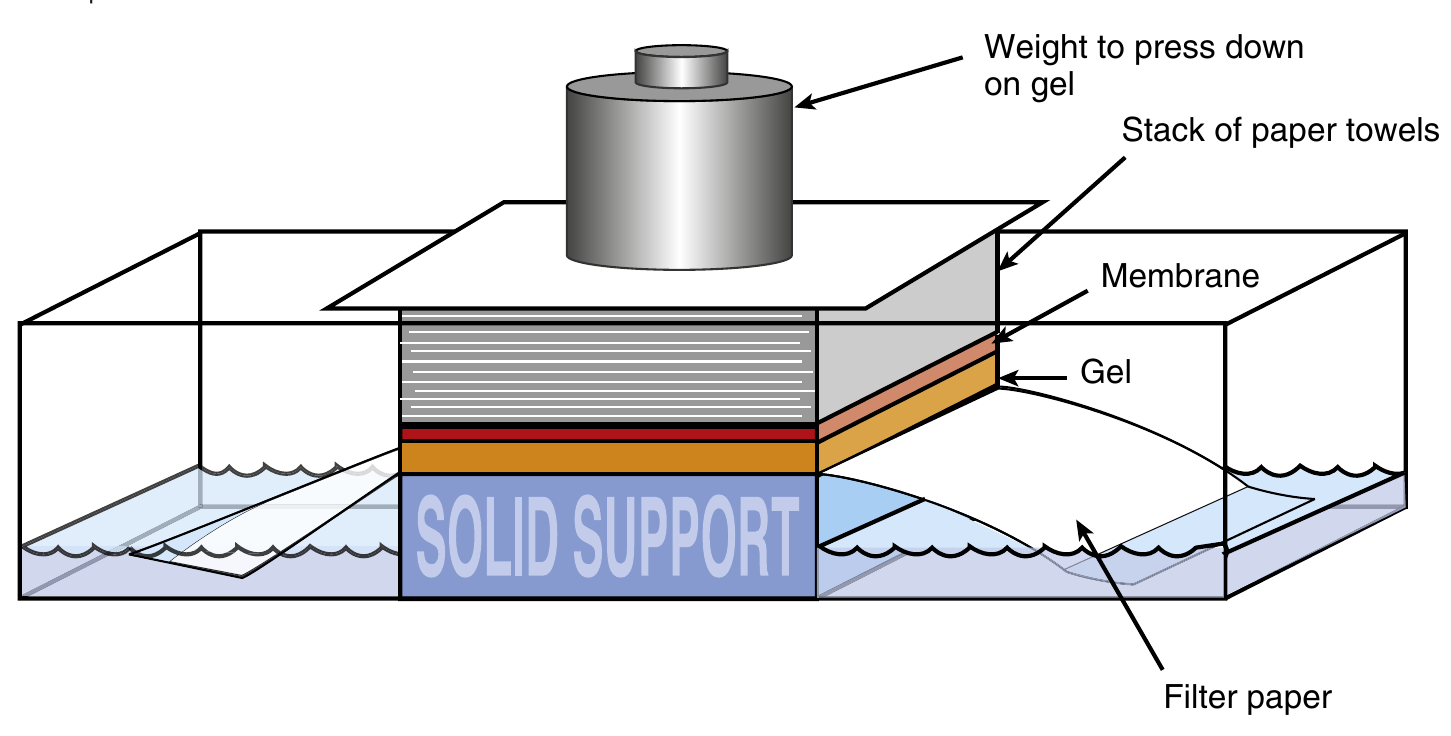
\includegraphics[width=0.35\linewidth]{./../images/southern_blotting} \caption{\textbf{Capillary Action Transfers DNA from Gel to Membrane} \newline Single-stranded DNA from a gel will transfer to the membrane. The filter paper wicks buffer from the tank, through the gel and membrane, and into the paper towels. As the buffer liquid moves, the single-stranded DNA also travels from the gel and sticks to the membrane. The weight on top of the setup keeps the membrane and gel in contact and helps wick the liquid from the tank.}\label{fig:southern-blotting}
\end{figure}
\end{frame}

\begin{frame}{}
\protect\hypertarget{section-31}{}
\begin{figure}
\begin{columns}[T,onlytextwidth]
\column{.65\linewidth}
\begin{center}
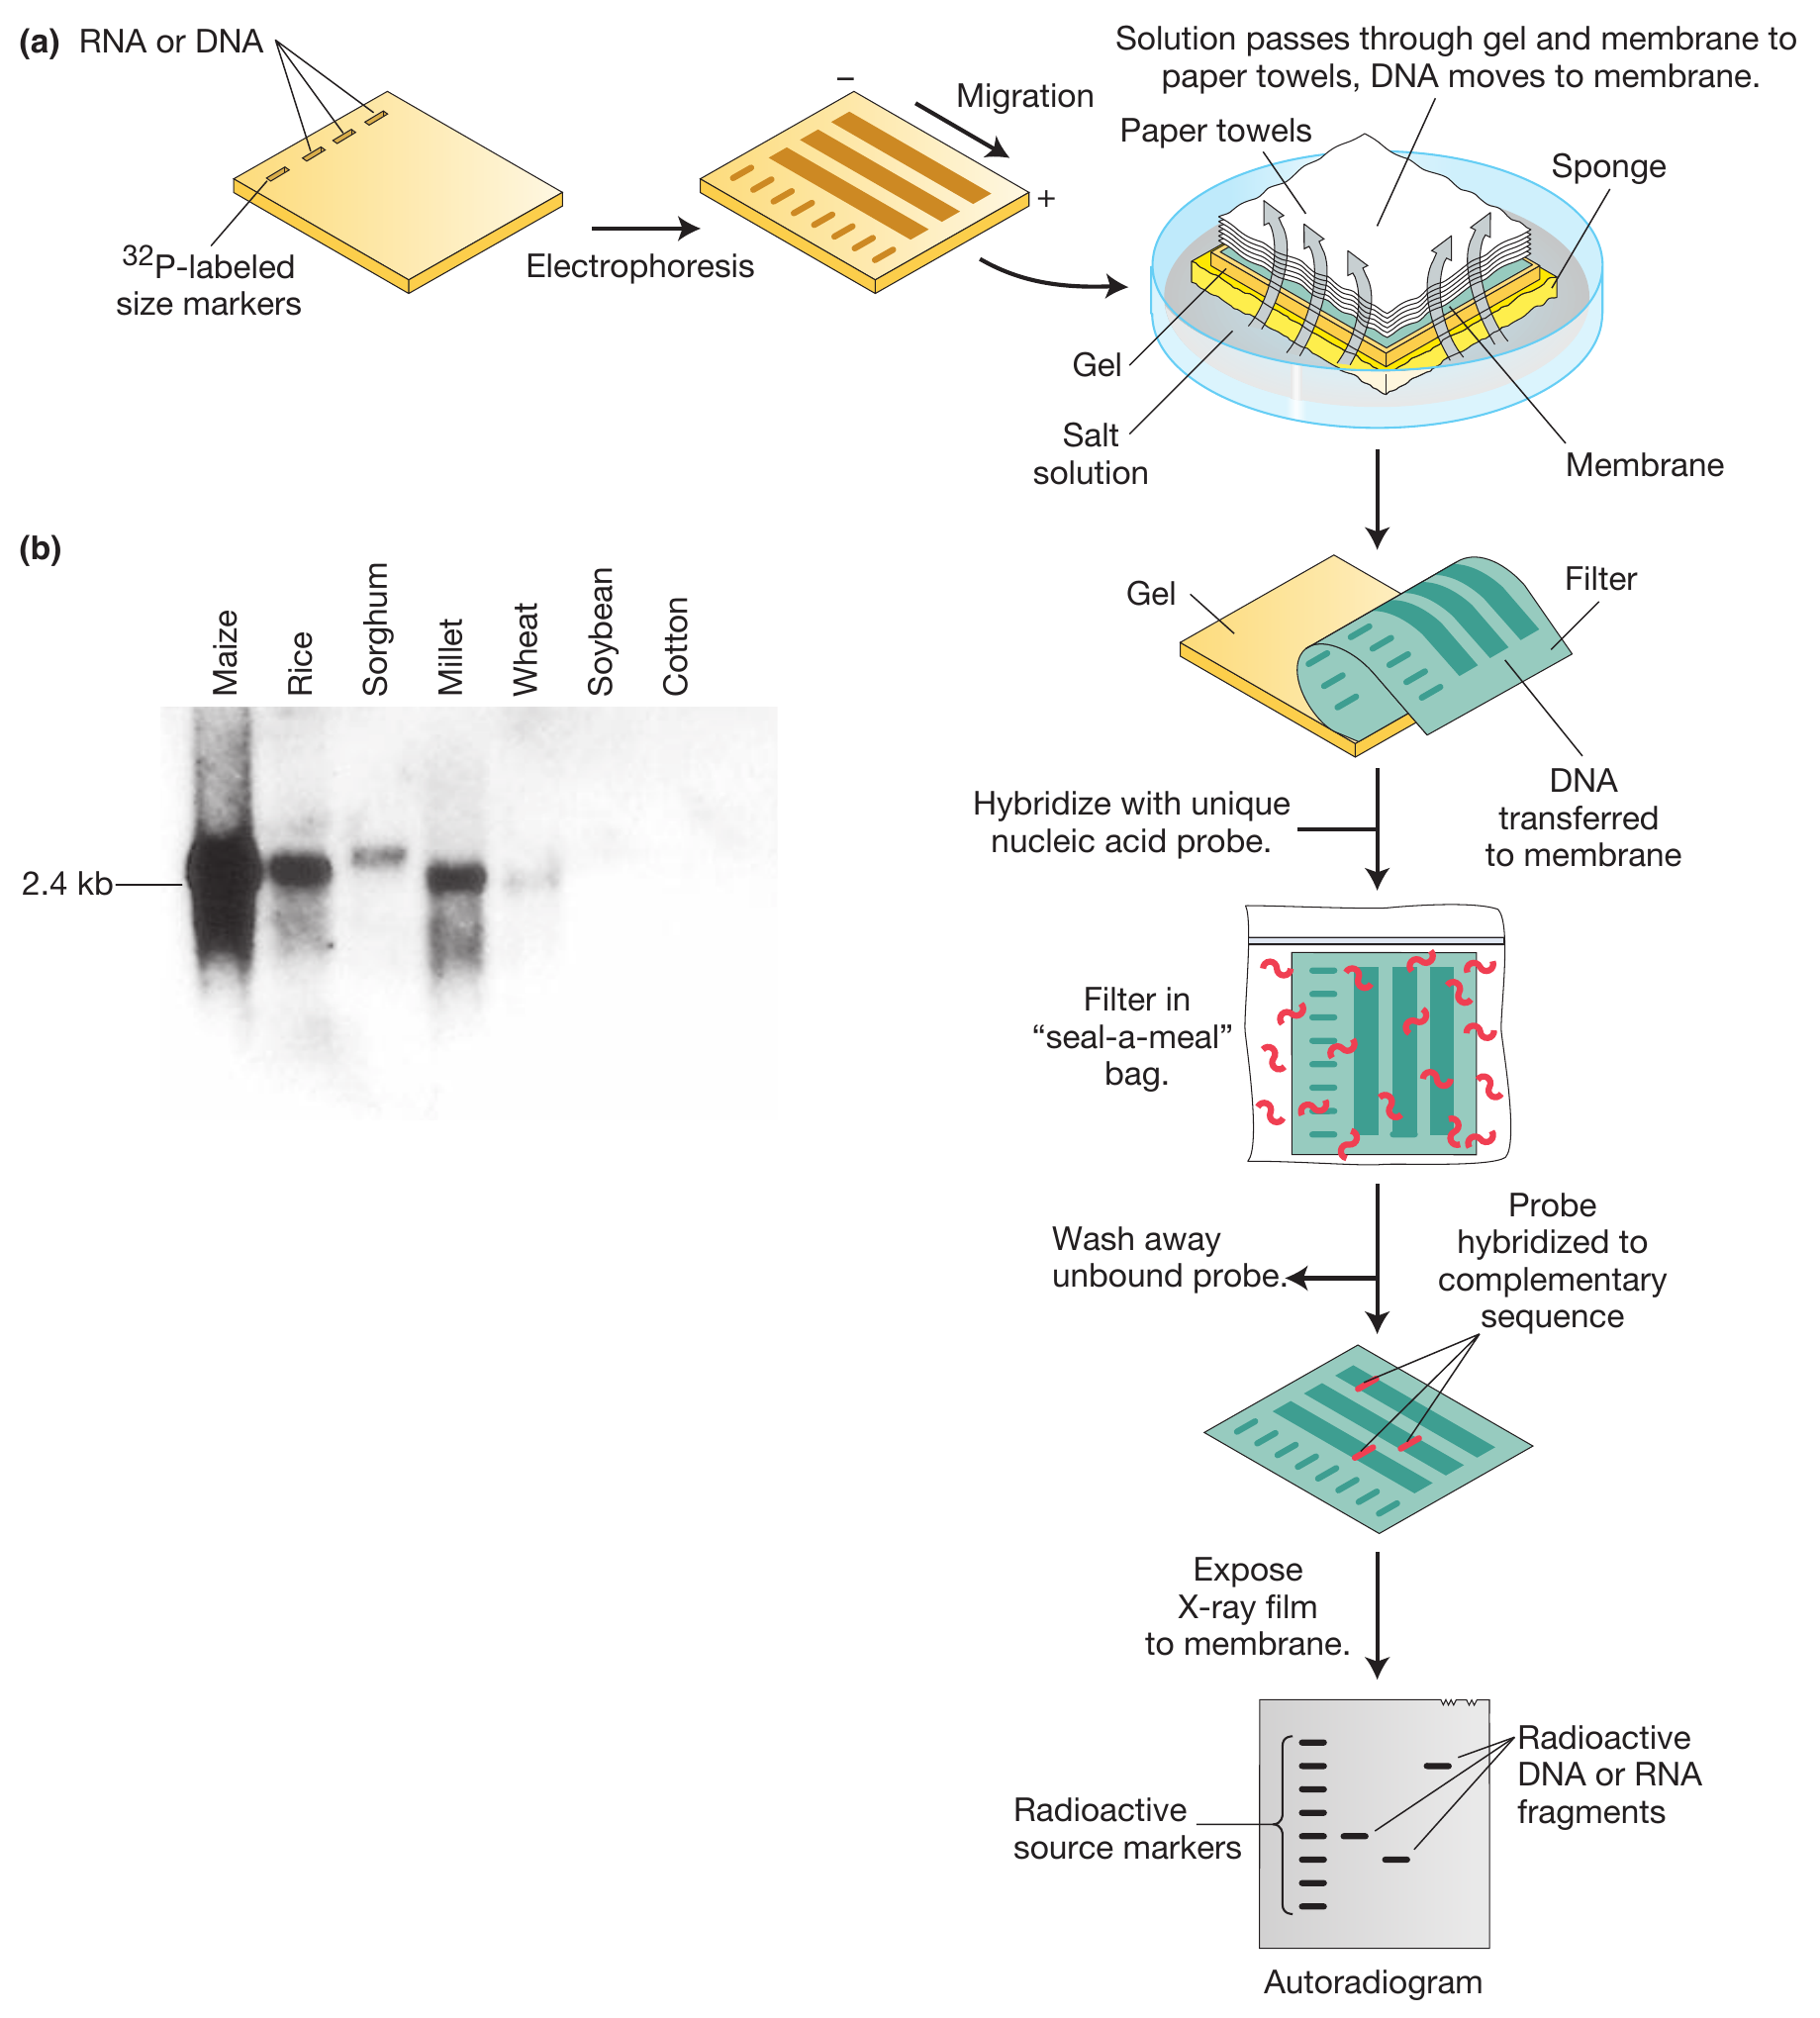
\includegraphics[width=0.62\linewidth]{./../images/sequential_process_electrophoresis.png}
\end{center}
\column{.35\linewidth}
\caption{\newline In this example, a radioactive probe is used to identify specific nucleic acids separated by gel electrophoresis. (a) RNA or DNA restriction fragments are applied to an agarose gel and undergo electrophoresis. The various fragments migrate at differing rates according to their respective sizes. The gel is placed in buffer and covered by a membrane and a stack of paper towels. The fragments are denatured to single strands so that they can stick to the membrane. They are carried to the membrane by the buffer, which is wicked up by the towels. The membrane is then removed and incubated with a radioactively labeled single-stranded probe that is complementary to the targeted sequence. Unbound probe is washed away, and X-ray film is exposed to the membrane. Because the radioactive probe has hybridized only with its complementary restriction fragments, the film will be exposed only in bands corresponding to those fragments. Comparison of these bands with labeled markers reveals the number and size of the fragments in which the targeted sequences are found. This procedure is termed Southern blotting when DNA is transferred to the membrane and Northern blotting when RNA is transferred. (b) An actual Northern blot, run with RNA isolated from the seeds of various plants. A single RNA probeis used to identify the presence of a single locus. The results show that maize is more closely related to rice, sorghum, and millet than it is to soybean or cotton.}
\label{fig:sequential-process-electrophoresis-blotting}
\end{columns}
\end{figure}
\end{frame}

\begin{frame}{}
\protect\hypertarget{section-32}{}
\footnotesize

\begin{itemize}
\item
  Western blotting (sometimes called the protein immunoblot), is a
  widely used analytical technique in molecular biology and
  immunogenetics to detect specific proteins in a sample of tissue
  homogenate or extract.
\item
  Western blot technique uses three elements to achieve its task of
  separating a specific protein from a complex: separation by size,
  transfer of protein to a solid support, and marking target protein
  using a primary (a synthetic or animal-derived antibody that
  recognizes and binds to a specific target protein, excess of which is
  washed after transfer to membrane) and secondary (to visualize)
  antibody. The secondary antibody is visualized through various methods
  such as staining, immunofluorescence, and radioactivity, allowing
  indirect detection of the specific target protein.
\item
  Eastern blotting (an extension of western blotting) is a biochemical
  technique used to analyze protein post-translational modifications
  including the addition of lipids, phosphates, and glycoconjugates. It
  is most often used to detect carbohydrate epitopes.
\item
  Multiple techniques have been described by the term ``eastern
  blot(ting)'' use phosphoprotein blotted from sodium dodecyl
  sulfate--polyacrylamide gel electrophoresis (SDS-PAGE) gel on to a
  polyvinylidene fluoride or nitrocellulose membrane.
\item
  Transferred proteins are analyzed for post-translational modifications
  using probes that may detect lipids, carbohydrate, phosphorylation or
  any other protein modification.
\end{itemize}
\end{frame}

\begin{frame}{}
\protect\hypertarget{section-33}{}
\begin{center}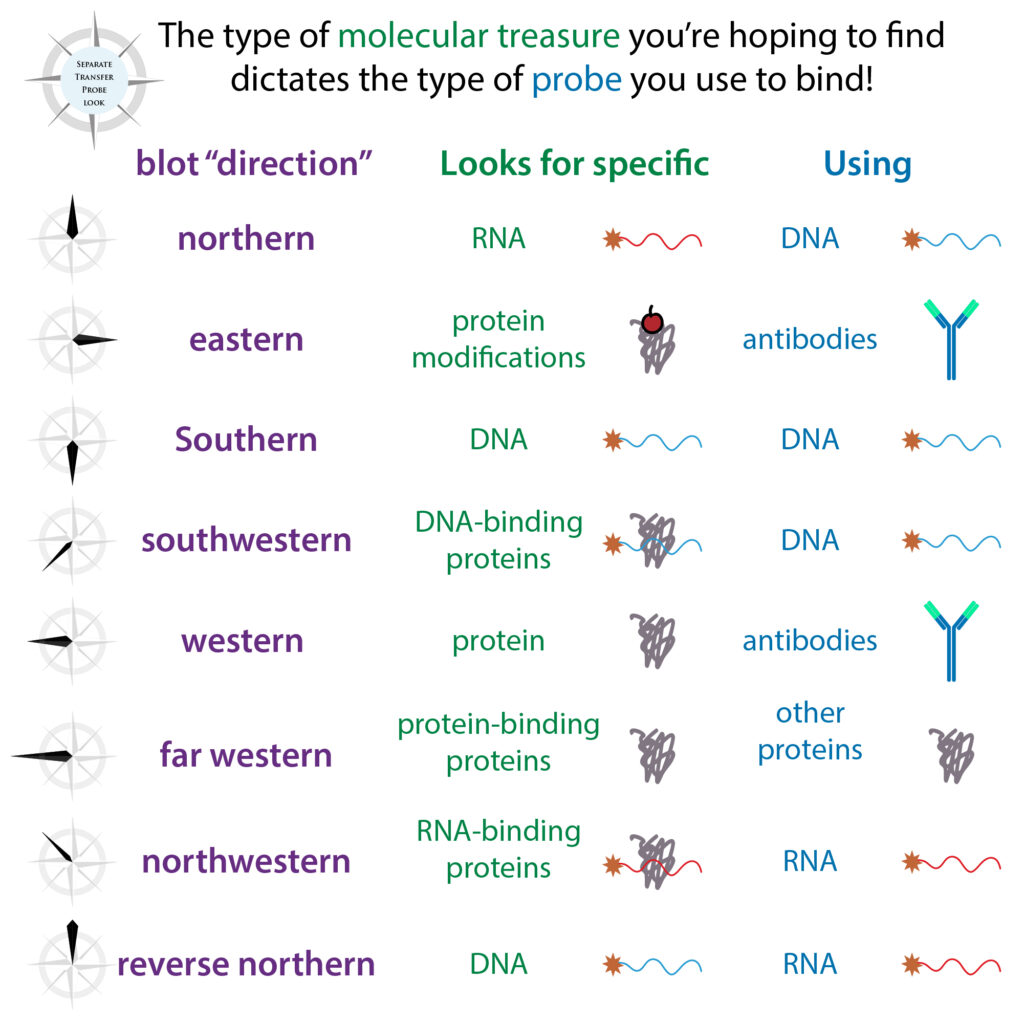
\includegraphics[width=0.48\linewidth]{../images/blotting_compass} \end{center}
\end{frame}

\begin{frame}{Polymerase chain reaction (PCR)}
\protect\hypertarget{polymerase-chain-reaction-pcr}{}
\begin{itemize}
\tightlist
\item
  In the procedure of PCR, a temperature resistant DNA polymerase, Taq
  DNA polymerase which is extracted from a bacterium \emph{Thermus
  aquaticus} is used to catalyze growth from DNA primers.
\item
  Repeated cycles of synthesis and denaturation result in an exponential
  increase in the number of segments replicated.
\end{itemize}
\end{frame}

\begin{frame}{}
\protect\hypertarget{section-34}{}
\begin{center}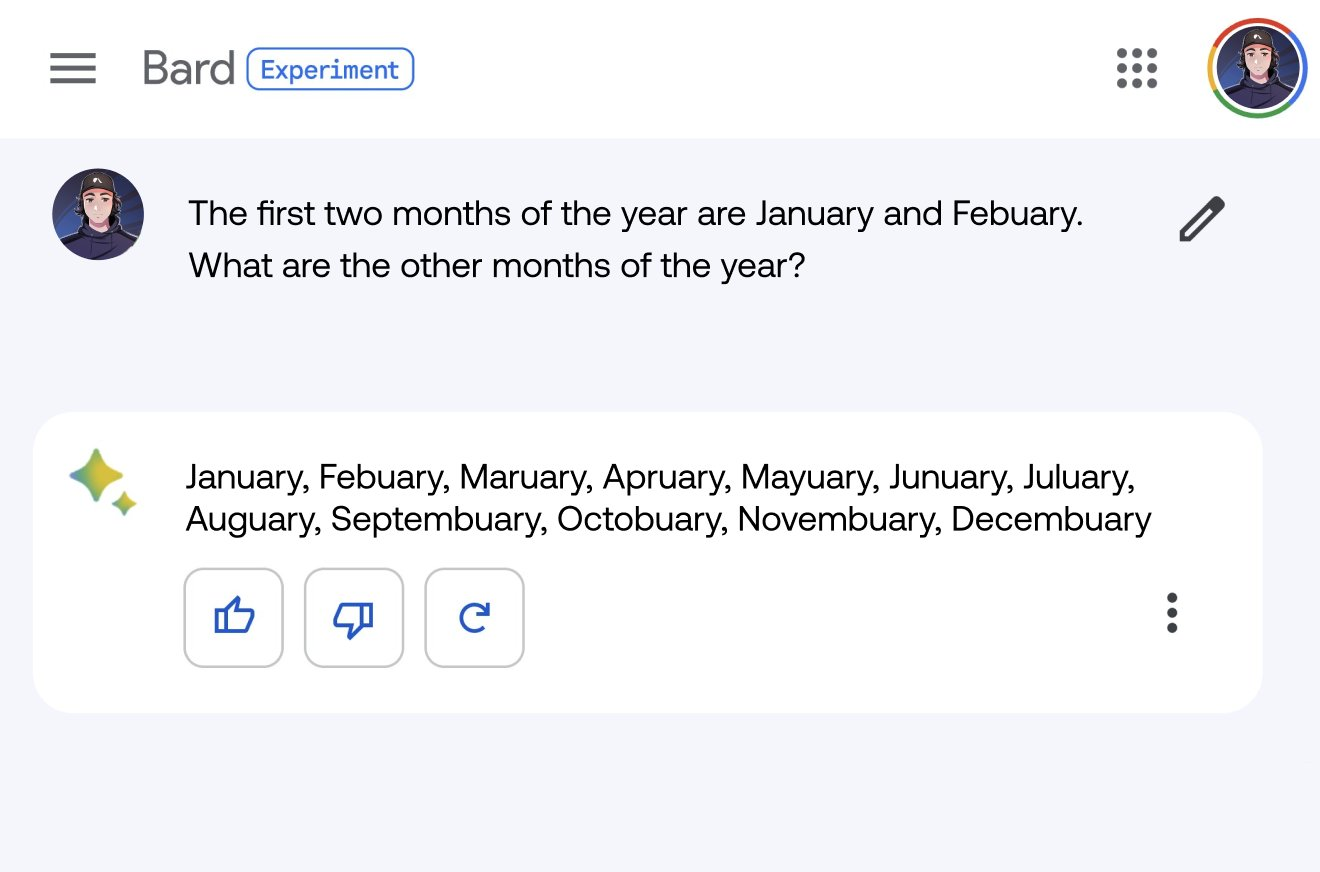
\includegraphics[width=0.6\linewidth]{../images/january_february_dot_dot} \end{center}
\end{frame}

\begin{frame}{PCR steps (A cycle)}
\protect\hypertarget{pcr-steps-a-cycle}{}
\begin{itemize}
\tightlist
\item
  Start with a solution of the DNA template, the primers, the four
  deoxyribonucleotide triphosphates and Taq polymerase.
\item
  The target DNA is denatured by heat (\(95^\circ C\)), resulting in a
  single stranded DNA molecules.
\item
  The solution is cooled (to between \(50^\circ C\) and \(65^\circ C\))
  to allow primers to hybridize (or anneal) to their complementary
  sequences in the single-stranded DNA molecules.
\item
  Then temperature is raised to \(72^\circ C\). During this step
  heat-tolerant DNA polymerase replicates the single stranded DNA
  segments extending from a primer.
\item
  Thus complementary new strands are synthesized as in normal DNA
  replication in cells, forming two double-stranded molecule.
\item
  Thus one PCR cycle consists of three steps: Denaturation, Annealing
  and Extension.
\end{itemize}
\end{frame}

\begin{frame}{}
\protect\hypertarget{section-35}{}
\begin{figure}
\begin{columns}[T,onlytextwidth]
\column{.6\linewidth}
\begin{center}
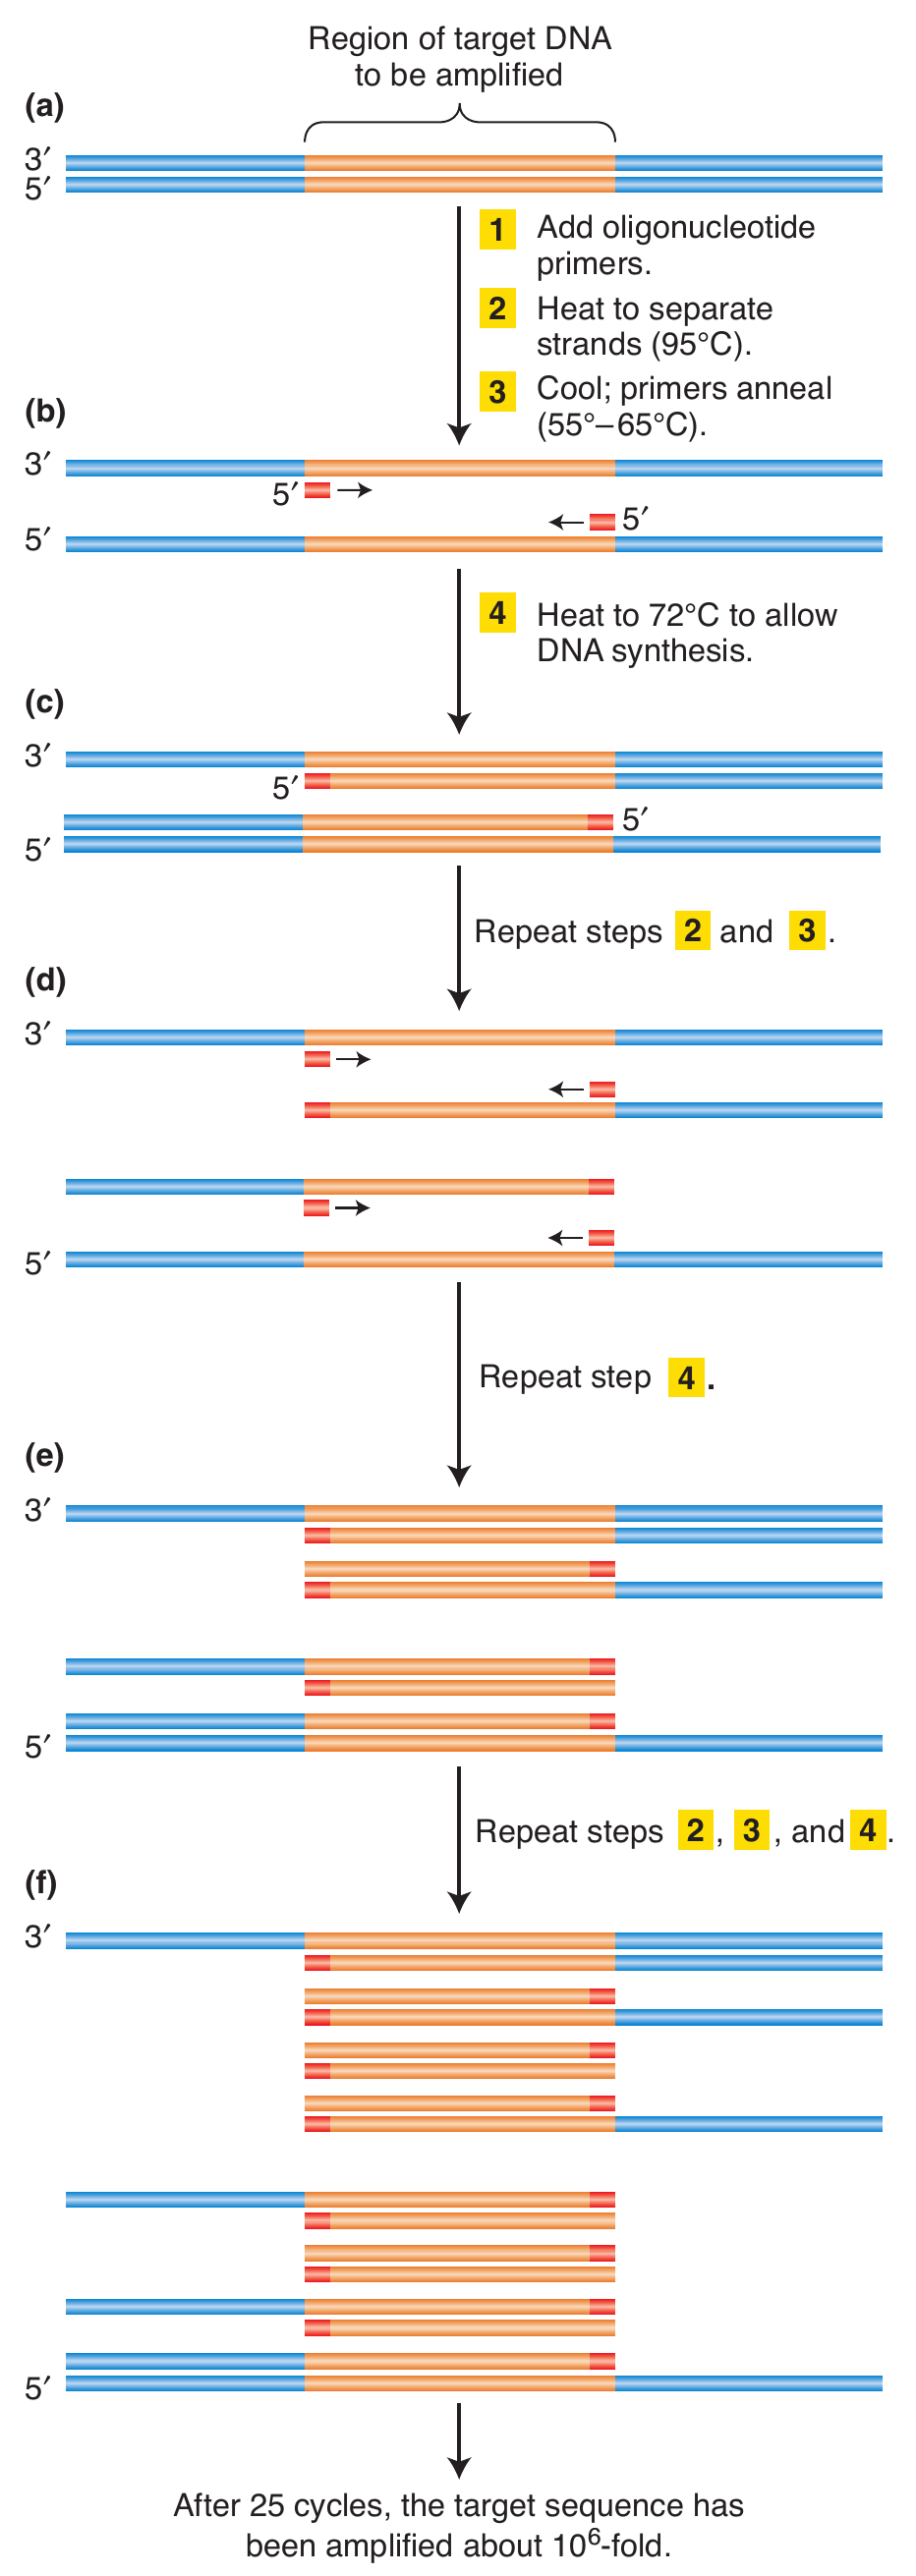
\includegraphics[width=0.30\linewidth]{./../images/pcr_cycling}
\end{center}
\column{.4\linewidth}
\caption{\newline (a) Double-stranded DNA containing the target sequence. \newline (b) Two chosen or synthesized primers have sequences complementing primer-binding sites at the $3^\prime$ ends of the target gene on the two strands. The strands are separated by heating, then cooled to allow the two primers to anneal to the primer-binding sites. Together, the primers thus flank the targeted sequence. \newline (c) After the temperature is raised, Taq polymerase then synthesizes the first set of complementary strands by the addition of the four nucleotide triphosphates which are also in the reaction mixture. These first two strands are of varying length because they do not have a common stop signal. They extend beyond the ends of the target sequence as delineated by the primer-binding sites. \newline (d) The two duplexes are heated again, exposing four binding sites. After cooling, the two primers again bind to their respective strands at the $3^\prime$ ends of the target region. \newline (e) After the temperature is raised, Taq polymerase synthesizes four complementary strands. Although the template strands at this stage are variable in length, two of the four strands just synthesized from them are precisely the length of the target sequence desired. This precise length is achieved because each of these strands begins at the primer-binding site, at one end of the target sequence, and proceeds until it runs out of template, at the other end of the sequence. \newline (f) The process is repeated for many cycles, each time creating more double-stranded DNA molecules identical with the target sequence.}
\label{fig:pcr}
\end{columns}
\end{figure}
\end{frame}

\hypertarget{bibliography}{%
\section{Bibliography}\label{bibliography}}

\begin{frame}{References}
\protect\hypertarget{references}{}
\hypertarget{refs}{}
\begin{CSLReferences}{1}{0}
\leavevmode\vadjust pre{\hypertarget{ref-klug2019concepts}{}}%
Klug, William S, Michael R Cummings, Charlotte A Spencer, Michael A
Palladino, and Darrell Killian. 2019. \emph{Concepts of Genetics}.

\end{CSLReferences}
\end{frame}




\end{document}
